\documentclass{ieeeaccess}

\usepackage{cite}
\usepackage{amsmath,amssymb,amsfonts}
\input{math_commands.tex}
\usepackage{amsthm}
\usepackage{mathtools}
\usepackage{booktabs}
\usepackage{longtable}
\usepackage{graphicx}
\usepackage{algorithm}
\usepackage{algpseudocode}
\usepackage{textcomp}
\usepackage{url}
\usepackage[hypertexnames=false]{hyperref}

\def\BibTeX{{\rm B\kern-.05em{\sc i\kern-.025em b}\kern-.08em
    T\kern-.1667em\lower.7ex\hbox{E}\kern-.125emX}}
\providecommand{\xfigwd}{0pt}
\makeatletter
\@ifundefined{c@biography}{\newcounter{biography}}{}
\@ifundefined{if@biographyTOCentrynotmade}{%
  \newif\if@biographyTOCentrynotmade
  \@biographyTOCentrynotmadetrue
}{}
\makeatother

\begin{document}

\history{Date of current version June 15, 2026.}
\doi{10.1109/ACCESS.2026.DOI}
\vol{14}
\Year{2026}

\title{Compute-Adaptive Risk Control: Finite-Sample Certificates for Early-Exit and Cascade Inference}

\author{\uppercase{Sooyoung Jang}\authorrefmark{1},
\uppercase{Sungpil Woo}\authorrefmark{1}, and
\uppercase{Ahyun Lee}\authorrefmark{2}}

\address[1]{Department of Computer Engineering, Hanbat National University,
Daejeon 34158, Republic of Korea (e-mail: syjang@hanbat.ac.kr; woosungpil@hanbat.ac.kr)}
\address[2]{Department of Intelligent Media Engineering, Hanbat National University,
Daejeon 34158, Republic of Korea (e-mail: ahyun@hanbat.ac.kr)}

\markboth
{S. Jang \headeretal Compute-Adaptive Risk Control}
{S. Jang \headeretal Compute-Adaptive Risk Control}

\corresp{Corresponding authors: Sungpil Woo (e-mail: woosungpil@hanbat.ac.kr) and Ahyun Lee (e-mail: ahyun@hanbat.ac.kr).}


\begin{abstract}
Adaptive inference systems---early-exit networks and model cascades---cut average computation by letting inputs terminate early, but their thresholds are usually chosen by inspecting a validation set. That step provides no finite-sample certificate that deployment risk stays below a target, because the same data both screen the candidate thresholds and pick the deployed policy. This paper studies \emph{compute-adaptive risk control} (CARC): threshold selection over a fixed, compute-ordered candidate family with the guarantee that the selected policy satisfies $R(\tau)\le\alpha$ with probability at least $1-\delta$ over the calibration draw. CARC instantiates Learn-then-Test with family-wise error control and contributes (i) a cost characterization for fixed-sequence certification on compute chains, (ii) a joint risk--compute certificate for pre-committed budgets, (iii) an estimated-weight sensitivity certificate for covariate shift, and (iv) a deployment discipline that separates validity from feasibility---reporting \emph{infeasibility} rather than attaching a guarantee to an uncertified fallback. A controlled simulation with oracle risks confirms the certificate while uncorrected tuning violates at far higher rates; a preregistered scikit-learn digits cascade confirms the procedure on a feasible real cache, where naive tuning still violates the target in up to $57\%$ of trials; and a CIFAR-100 branchy cache documents correct infeasibility reporting where the trained model cannot meet its targets but naive tuning would deploy an unsafe policy.
\end{abstract}

\begin{keywords}
Adaptive inference, calibration, early-exit networks, finite-sample guarantees, risk control, statistical learning.
\end{keywords}

\titlepgskip=-15pt
\maketitle

\section{Introduction}

Adaptive-depth inference --- early-exit networks, cascades, and routers --- trades accuracy for latency, energy, and operating cost by allowing inputs to terminate before the most expensive model path. The usual deployment procedure is straightforward: train the adaptive model, evaluate candidate thresholds on held-out data, and deploy the cheapest threshold whose empirical risk appears acceptable. The missing step is statistical certification after threshold selection. Because the same calibration statistic is used both to screen candidates and to choose the deployed policy, the selected threshold can have true risk above the target even when its empirical risk is below the target. A second gap is operational: when no threshold is safe for the trained system and target, the procedure should report infeasibility rather than returning a policy whose risk status is unknown.

This paper asks a specific question: \textbf{given a fixed adaptive inference system, a finite calibration set, a risk target $\alpha$, and an error probability $\delta$, can one select a compute-efficient threshold policy while controlling the probability of deploying an unsafe policy?} We answer this question by instantiating the Learn-then-Test (LTT) framework for compute-ordered threshold families \cite{angelopoulos2025learn}. The reduction from risk control to hypothesis testing is inherited from LTT; the contribution here is to connect that reduction to the structure of adaptive inference, where candidate policies are naturally ordered by compute and where infeasibility must be visible to an operator.

The empirical objective is correspondingly narrow. We do not claim state-of-the-art accuracy for any backbone. Instead, we test whether the certificate controls the frequency of unsafe selections, quantify the compute premium relative to uncorrected validation tuning, and record infeasibility when the trained system cannot meet the target. In the controlled simulation, where oracle risks are available, the certified chain stays below the tested violation levels while the invalid naive policy violates at $0.231$--$0.351$. In the preregistered digits real-cache study, the final exit is below the target grid before calibration and the chain again stays within the tested violation levels; at $\alpha=0.10$, naive validation inspection violates at $0.486$--$0.571$. The CIFAR-100 branchy-cache run is intentionally reported as a diagnostic feasibility case: the preregistered targets are mostly infeasible because the minimum full-pool chain risk is $0.3055$, and the feasible-target cells are exploratory.

\textbf{Scope of evidence.} The guarantees in Sections~3--6 are proved in Appendix A. The $1-\delta$ behavior and the failure mode of naive tuning are verified in a controlled simulation with oracle risks (Section~10.1). A preregistered tabular real-cache study on the scikit-learn digits data gives the positive real-cache confirmation (Section~10.2); because CARC operates only on cached scores, losses, and costs, this non-neural staged cascade exercises the calibration layer end-to-end on a feasible target grid without standing in for a deep early-exit network. The CIFAR-100 branchy network is the neural early-exit case, used to stress infeasibility reporting (Section~10.3). Larger ImageNet, language-cascade, and real-shift deployments are future work rather than evidence for the present claims.

Figure~\ref{fig:pipeline} summarizes the deployment logic before the formal notation. The model is fixed before calibration; CARC uses the calibration cache only to certify a pre-specified chain, while the naive branch inspects the same cache without a family-wise risk certificate.

\begin{figure}[t]
\centering
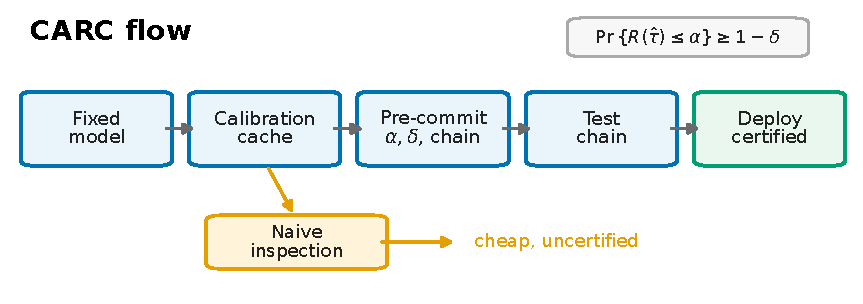
\includegraphics[width=\linewidth]{figures/fig1_pipeline.pdf}
\caption{\textbf{CARC calibration/deployment flow.} A fixed multi-exit model produces cached calibration scores, losses, and compute values. The user pre-commits $(\alpha,\delta)$ and a compute-ordered chain; LTT-style tests certify configurations from expensive to cheap; the deployed policy is the cheapest certified one, or the procedure reports infeasibility. The orange branch shows the naive validation-inspection baseline: it may be cheap, but it does not provide the family-wise certificate used for risk control.}
\label{fig:pipeline}
\end{figure}

\subsection{Contributions}

The reduction "risk control = multiple testing" and the admissibility of fixed-sequence and graphical tests are due to LTT and the multiple-testing literature. This paper contributes the following components.

\begin{enumerate}
\item \textbf{Finite-family formulation for adaptive inference.} We cast threshold selection for early-exit and cascade policies as risk control over a finite, compute-ordered candidate family. The formulation applies to any bounded loss $\ell_{\mathrm{loss}}\in[0,1]$, including 0--1 error, selective risk, and class-conditional error rates.
\item \textbf{Cost characterization for fixed-sequence certification.} The validity guarantee is inherited from LTT and carries no chain-length penalty. The new statement in Theorem 2(b) is an efficiency characterization: under a monotone-risk condition, the selected policy lies within a finite-sample boundary band of the cheapest safe policy in the chosen chain, with width $\Delta_n=O(\sqrt{\ln(K/\delta)/n})$.
\item \textbf{Joint risk--compute certificate.} Theorem 3 certifies $R(\tau)\le\alpha$ and $C(\tau)\le B$ for settings where a compute budget must be fixed before deployment. The risk certificate remains the primary guarantee; the compute certificate is a conservative pre-commitment device rather than a substitute for measuring realized latency.
\item \textbf{Estimated-weight shift certificate.} Theorem 4 gives a finite-sample sufficient condition under covariate shift when importance weights are estimated on a separate fold and an $L^1$ error budget $\eta$ is supplied. The result is a sensitivity certificate: validity depends on the correctness of the budget, and feasibility can degrade as $\eta$ increases.
\item \textbf{Certify-or-report-infeasibility deployment discipline.} We separate three quantities that validation tuning conflates---risk validity, feasibility of the target for the trained system, and compute efficiency---and require the procedure to report \emph{infeasibility} rather than attach a risk guarantee to an uncertified fallback. The CIFAR-100 study is included as a documented instance of this discipline under stress: where no preregistered target admits a safe configuration, CARC certifies nothing and reports infeasibility, whereas uncorrected validation tuning selects an unsafe policy in $28$--$46\%$ of trials and violates the target in exactly those trials. Reporting this negative outcome faithfully is part of the contribution, not a shortfall of it.
\item \textbf{Implementation and validation.} The reference implementation covers the p-values, certification procedures, selectors, and cache evaluators. Experiments verify the guarantee in a simulation with oracle risks, confirm the real-cache procedure on a feasible digits cascade, and document infeasibility reporting on a CIFAR-100 branchy cache whose preregistered targets are mostly unattainable.
\end{enumerate}

\subsection{Relation to Learn-then-Test}

\emph{Borrowed.} From LTT \cite{angelopoulos2025learn} and the multiple-testing literature \cite{holm1979simple,wiens2003fixed,bretz2008graphical}, we use the reduction from risk control to testing nulls $H_\tau:R(\tau)>\alpha$, valid concentration p-values, and family-wise error rate (FWER) procedures for finite hypothesis families. The Hoeffding--Bentkus and empirical-Bernstein p-values are also standard ingredients \cite{hoeffding1963probability,bentkus2004hoeffding,maurer2009empirical}.

\emph{New.} We specialize this machinery to adaptive inference and analyze what the compute order buys. Theorem 2(b) characterizes the efficiency loss of fixed-sequence certification on an exit/cascade chain; Theorem 3 adds a conservative joint risk--compute certificate for pre-committed budgets; Theorem 4 gives an estimated-weight sufficient condition for covariate shift; and the implementation evaluates these claims with controlled simulation, digits real-cache confirmation, and CIFAR-100 feasibility diagnostics. The contribution is therefore not a new multiple-testing method, but a calibrated threshold-selection methodology for compute-adaptive inference. When the chain order is doubtful, we implement Holm's step-down procedure \cite{holm1979simple}; the graphical family in \cite{bretz2008graphical} is a broader unimplemented option.

\begin{table}[t]
\centering
\caption{What CARC borrows from Learn-then-Test (LTT) and the multiple-testing literature, and what it adds. The validity machinery is inherited; the new content is the compute-chain specialization and the certificates and deployment semantics built on it.}
\label{tab:ltt-delta}
\scriptsize
\setlength{\tabcolsep}{4pt}
\begin{tabular}{@{}p{4.0cm}lp{2.3cm}@{}}
\toprule
Ingredient & Source & Role in CARC \\
\midrule
Risk control $=$ multiple testing & Borrowed & Foundation \\
Concentration p-values (Hoeffding, HB, emp.\ Bernstein) & Borrowed & Per-config tests \\
FWER rules (Bonferroni, fixed-sequence, Holm) & Borrowed & Certification \\
Compute-ordered chain from exit structure & New & Supplies test order \\
Two-sided cost bound (Th.~2(b)) & New & Efficiency band \\
Joint risk--compute certificate (Th.~3) & New & Pre-committed budget \\
Estimated-weight shift certificate (Th.~4) & New & Shift sensitivity \\
Certify-or-report-infeasibility & New & Deployment semantics \\
\bottomrule
\end{tabular}
\end{table}

\section{Problem setup and notation}

Let $(X,Y)\sim P$ with $X\in\mathcal X$, $Y\in\mathcal Y$. A multi-exit network has exits $\ell\in\{1,\dots,L\}$ ordered by depth. Exit $\ell$ produces a prediction $\hat y_\ell(x)$ and a scalar confidence $s_\ell(x)\in[0,1]$ (e.g., top softmax probability, or $1-$ entropy). Let $c_\ell\ge0$ be the cumulative compute (FLOPs, or wall-clock proxy) to \emph{reach and evaluate} exit $\ell$, with $c_1<c_2<\dots<c_L=:C_{\max}$.

\textbf{Exit policy.} A configuration is a threshold vector $\tau=(\tau_1,\dots,\tau_{L-1})\in[0,1]^{L-1}$. On input $x$, the policy exits at

\[
E_\tau(x)=\min\big(\{\,\ell<L : s_\ell(x)\ge\tau_\ell\,\}\cup\{L\}\big),
\]

i.e., it stops at the first exit whose confidence clears its threshold, and otherwise runs to the final exit $L$. The deployed prediction is $\hat Y_\tau(x)=\hat y_{E_\tau(x)}(x)$.

\textbf{Risk and compute functionals.} For a bounded loss $\ell_{\mathrm{loss}}:\mathcal Y\times\mathcal Y\to[0,1]$,

\[
R(\tau) \;=\; \mathbb E_{P}\!\big[\ell_{\mathrm{loss}}(\hat Y_\tau(X),Y)\big],
\qquad
C(\tau) \;=\; \mathbb E_{P}\!\big[c_{E_\tau(X)}\big].
\]

Examples of $\ell_{\mathrm{loss}}$: 0--1 error $\mathbf 1\{\hat Y_\tau\ne Y\}$; selective risk on accepted points; class-conditional false-negative rate (clip to $[0,1]$). All that the theory needs is boundedness.

\textbf{Calibration data.} We observe $n$ i.i.d. draws $\mathcal D=\{(X_i,Y_i)\}_{i=1}^n\sim P$, disjoint from training. Define empirical estimates

\[
\hat R(\tau)=\frac1n\sum_{i=1}^n \ell_{\mathrm{loss}}(\hat Y_\tau(X_i),Y_i),
\qquad
\hat C(\tau)=\frac1n\sum_{i=1}^n c_{E_\tau(X_i)}.
\]

\textbf{Goal.} Given target risk $\alpha\in(0,1)$ and confidence level $\delta\in(0,1)$, return $\hat\tau$ (a measurable function of $\mathcal D$) such that

\begin{equation}
\Pr_{\mathcal D}\big(R(\hat\tau)\le\alpha\big)\;\ge\;1-\delta,
\tag{P1}
\end{equation}

and, among configurations satisfying (P1), $\hat\tau$ has small compute $C(\hat\tau)$. A stronger \emph{dual} specification adds a budget $B$:

\begin{equation}
\Pr_{\mathcal D}\big(R(\hat\tau)\le\alpha \ \text{and}\ C(\hat\tau)\le B\big)\ge 1-\delta.
\tag{P2}
\end{equation}

\textbf{Grid.} We work over a finite candidate set $\Lambda\subset[0,1]^{L-1}$ (e.g., a per-exit grid of $m$ thresholds, $|\Lambda|\le m^{L-1}$, or a scalar-parameterized chain; see Section~4). All probabilities below are over the draw of $\mathcal D$; $\hat\tau$ is data-dependent.

\textbf{Nature of the guarantee.} (P1) is a \emph{training-conditional} (PAC-style) statement: with probability $\ge1-\delta$ over the calibration draw, the \emph{fixed, deployed} policy $\hat\tau$ has true risk $\le\alpha$ for all subsequent inputs. It is not a marginal-over-future-test-points guarantee that averages away calibration noise; it is the stronger object an operator wants, since $\hat\tau$ is frozen at deployment. The qualifier \emph{distribution-free} applies to \textbf{validity}: it holds for any $P$. It does \textbf{not} extend to the efficiency (cost-optimality) and shift results, which require, respectively, a monotonicity condition (Section~4.1) and a weight-error budget (Section~6.2); we flag this wherever it matters.

\section{Risk control as multiple testing}

We adapt Learn-then-Test (LTT) \cite{angelopoulos2025learn}. For each $\tau\in\Lambda$ define the null

\[
H_\tau:\quad R(\tau)>\alpha \quad(\text{``}\tau\text{ is unsafe''}).
\]

Rejecting $H_\tau$ certifies $\tau$ as safe. We need (a) a valid p-value $p_\tau$ for each $H_\tau$, and (b) a family-wise-error-controlling (FWER) procedure that maps $\{p_\tau\}$ to a certified set $\hat\Lambda\subseteq\Lambda$ with

\begin{equation}
\Pr\big(\exists\,\tau\in\hat\Lambda:\ R(\tau)>\alpha\big)\le\delta.
\tag{1}
\end{equation}

Given (1), \emph{any} selection rule restricted to $\hat\Lambda$ inherits validity, because the bad event "we output an unsafe $\tau$" is contained in "$\hat\Lambda$ contains an unsafe $\tau$."

\subsection{Valid p-values from concentration}

Because $\ell_{\mathrm{loss}}\in[0,1]$ and the $n$ losses are i.i.d. given $\tau$, $\hat R(\tau)$ is a mean of bounded i.i.d. variables. The one-sided Hoeffding inequality \cite{hoeffding1963probability} gives, for the boundary mean $R(\tau)=\alpha$ and any observed $\hat R(\tau)\le\alpha$,

\[
\Pr_{R(\tau)=\alpha}\!\big(\hat R(\tau)\le \hat r\big)\;\le\;\exp\!\big(-2n(\alpha-\hat r)^2\big).
\]

Since under $H_\tau$ we have $R(\tau)\ge\alpha$ (taking the closure), the supremum of the left side over the null is attained at $R(\tau)=\alpha$. Hence

\begin{equation}
\boxed{\,p_\tau \;=\; \exp\!\big(-2n\,(\alpha-\hat R(\tau))_+^2\big)\,}
\tag{2}
\end{equation}

is a valid (super-uniform under $H_\tau$) p-value, where $(z)_+=\max(z,0)$. Tighter choices---the \textbf{Hoeffding--Bentkus (HB)} p-value used in LTT \cite{angelopoulos2025learn,bentkus2004hoeffding}, or an empirical-Bernstein p-value \cite{maurer2009empirical} when the loss has small variance---slot in directly and improve power; we use (2) for exposition and HB in experiments.

\subsection{Bonferroni LTT (assumption-free baseline)}

Reject $H_\tau$ iff $p_\tau\le\delta/|\Lambda|$, giving $\hat\Lambda_{\mathrm{Bonf}}=\{\tau:p_\tau\le\delta/|\Lambda|\}$. Then output

\[
\hat\tau=\arg\min_{\tau\in\hat\Lambda_{\mathrm{Bonf}}}\hat C(\tau)
\quad\text{if }\hat\Lambda_{\mathrm{Bonf}}\ne\varnothing,
\]
and otherwise report infeasibility for the requested $(\alpha,\delta,n,\Lambda)$ without issuing a certified deployment policy.

\textbf{Theorem 1 (Distribution-free risk validity).} \emph{For losses in $[0,1]$, i.i.d. calibration data, p-values (2), and the Bonferroni rule at level $\delta$, the probability that the procedure certifies and outputs an unsafe configuration is at most $\delta$: $\Pr(\text{output exists and }R(\hat\tau)>\alpha)\le\delta$. If the certified set is empty, it reports infeasibility rather than claiming a risk guarantee.}

\emph{Proof.} By Bonferroni, $\Pr(\exists\tau\in\hat\Lambda_{\mathrm{Bonf}}:R(\tau)>\alpha)\le\sum_{\tau:R(\tau)>\alpha}\Pr(p_\tau\le\delta/|\Lambda|)\le |\{\tau:H_\tau\}|\cdot \delta/|\Lambda|\le\delta$, using super-uniformity of $p_\tau$ under $H_\tau$. On the complementary event every certified $\tau$ is safe; if the procedure outputs, $\hat\tau\in\hat\Lambda_{\mathrm{Bonf}}$, so $R(\hat\tau)\le\alpha$. If $\hat\Lambda_{\mathrm{Bonf}}=\varnothing$, the procedure reports infeasibility and no certified-risk statement is attached to any operational fallback unless that fallback is separately certified. $\square$

The defect of Bonferroni is the $\delta/|\Lambda|$ penalty: with a fine per-exit grid $|\Lambda|$ is large, the threshold is tiny, and the certified set is small and expensive. The next section avoids this penalty on the \emph{validity} side by testing a pre-ordered chain --- at the price of restricting the search to that chain, a trade-off we make explicit.

\section{The compute-chain instantiation}

Fixed-sequence testing is a standard FWER procedure, already named in LTT for monotone, pre-orderable hypotheses \cite{angelopoulos2025learn,wiens2003fixed}; this section does \textbf{not} propose it as new. What it contributes is that early-exit deployment supplies the pre-specified order without extra design, aligned with the deployment objective, plus a two-sided cost bound (Theorem 2(b)) on how close the resulting policy is to the cheapest safe policy in the chain.

\subsection{The monotone structure of exit policies}

Order configurations by \textbf{compute}. Consider a \emph{chain} of configurations $\tau^{(1)}\preceq\tau^{(2)}\preceq\dots\preceq\tau^{(K)}$ that is increasing in compute, i.e. $C(\tau^{(1)})\le\dots\le C(\tau^{(K)})$, with $\tau^{(K)}=\mathbf 1$ the always-run-to-$L$ policy. A natural and common construction is a \textbf{scalar-parameterized} family $\tau(t)=(t,\dots,t)$ for $t$ on a grid $0=t_1<\dots<t_K=1$: raising the global threshold $t$ makes every exit more conservative, pushing more inputs to deeper exits, which \emph{increases} compute monotonically (deterministically, since each input's exit index is nondecreasing in $t$). More refined chains (per-exit thresholds raised in a fixed schedule) are also admissible.

\textbf{Assumption M (monotone risk along the chain).} $R(\tau^{(1)})\ge R(\tau^{(2)})\ge\dots\ge R(\tau^{(K)})$; equivalently, deeper-on-average policies have weakly lower risk.

Assumption M says deeper exits are, on average, at least as accurate --- the premise that motivates deploying a deep model at all. Its empirical version (monotone $\hat R$ along the chain) is observable, and we report it; the assumption itself concerns the true $R$. Crucially, Assumption M is needed only for the \emph{efficiency} statement of Theorem 2(b), never for validity.

\textbf{Within-chain scope.} A chain is a one-dimensional curve through the $(L{-}1)$-dimensional configuration space, and the scalar family $\tau(t)=(t,\dots,t)$ in particular is restrictive: per-exit thresholds can dominate a single shared threshold. Consequently "cheapest safe policy" in Theorem 2 means cheapest \emph{along the chosen chain}, not the global optimum over all of $[0,1]^{L-1}$. The chain is a deliberate design choice trading search breadth against the multiplicity penalty: a Holm step-down over the full grid recovers more configurations at a $\log|\Lambda|$ cost (Section~4.2, remark), and the more general graphical family is a possible extension. We report the chain and Holm variants and let the practitioner pick between those implemented procedures.

\subsection{Certification along the chain}

Apply LTT's fixed-sequence test to the compute chain, walking from most expensive to cheapest, $\tau^{(K)},\tau^{(K-1)},\dots$, and \textbf{stopping at the first configuration that fails to certify}. With the Hoeffding p-value (2), the certification test $p_{\tau^{(k)}}\le\delta$ is exactly

\[
\hat R(\tau^{(k)})\;\le\;\alpha-\epsilon_n(\delta),
\qquad
\epsilon_n(\delta):=\sqrt{\tfrac{\ln(1/\delta)}{2n}} .
\]

Let $k^\star$ be the cheapest index reached before stopping; output $\hat\tau=\tau^{(k^\star)}$ if at least one configuration certifies. If even $\tau^{(K)}$ fails to certify, report the task infeasible at this $(\alpha,\delta,n)$ and do not claim a certified deployment policy. Running $\tau^{(K)}=\mathbf 1$ can be a conservative engineering fallback, but it is not a risk guarantee unless $\tau^{(K)}$ itself certifies or is separately known to satisfy $R(\tau^{(K)})\le\alpha$.

Define the cheapest truly-safe index $k_0:=\min\{k:R(\tau^{(k)})\le\alpha\}$.

\textbf{Theorem 2 (validity and a two-sided cost bound).}

\emph{(a) Validity (LTT/fixed-sequence; stated for completeness).} For p-values valid under each $H_{\tau^{(k)}}$ and the fixed-sequence rule at level $\delta$ on the pre-specified chain order, the probability of certifying and outputting an unsafe configuration is at most $\delta$, with no dependence on $K$.

\emph{(b) Cost bound (our contribution).} On the validity event the output never undercuts the safe frontier: $C(\hat\tau)\ge\min_{k:R(\tau^{(k)})\le\alpha}C(\tau^{(k)})$, and under Assumption M this means $k^\star\ge k_0$. For the other direction, let

\[
\Delta_n:=\epsilon_n(\delta)+\epsilon_n(\delta/K)=O\!\Big(\sqrt{\tfrac{\ln(K/\delta)}{n}}\Big),
\qquad
k_1:=\min\{k:\ R(\tau^{(j)})\le\alpha-\Delta_n\ \text{for all}\ j\ge k\}.
\]

Then $\Pr(k^\star\le k_1)\ge1-\delta$. Combining, on an event of probability $\ge1-2\delta$,

\[
k_0\ \le\ k^\star\ \le\ k_1,
\]

so the excess compute of the certified policy over the cheapest safe policy in the chain is at most $C(\tau^{(k_1)})-C(\tau^{(k_0)})$ --- the compute spanned by configurations whose true risk lies in the boundary band $(\alpha-\Delta_n,\,\alpha]$. As $n\to\infty$, $\Delta_n\to0$ and $k_1\to k_0$.

\emph{Proof.} (a) is the standard fixed-sequence guarantee: since the order is fixed in advance and we stop at the first non-rejection, an error (certifying and outputting an unsafe config) requires rejecting the first true null in the walk, which has probability $\le\delta$ by super-uniformity; this is independent of $K$.

(b) \emph{Lower bound.} $\hat\tau$ is certified, hence safe on the validity event, so its compute is at least that of the cheapest safe configuration; under Assumption M the safe set is the suffix $\{k\ge k_0\}$ and compute is increasing in $k$, giving $k^\star\ge k_0$. \emph{Upper bound.} The walk reaches index $k_1$ iff every config in $\{k_1,\dots,K\}$ certifies, i.e. $\hat R(\tau^{(j)})\le\alpha-\epsilon_n(\delta)$ for all $j\ge k_1$. For any such $j$, $R(\tau^{(j)})\le\alpha-\Delta_n=\alpha-\epsilon_n(\delta)-\epsilon_n(\delta/K)$, so

\[
\Pr\big(\hat R(\tau^{(j)})>\alpha-\epsilon_n(\delta)\big)\le\Pr\big(\hat R(\tau^{(j)})-R(\tau^{(j)})>\epsilon_n(\delta/K)\big)\le e^{-2n\,\epsilon_n(\delta/K)^2}=\delta/K
\]

by the upper-tail Hoeffding inequality. A union bound over the at most $K$ such indices gives $\Pr(\exists j\ge k_1:\ \hat R(\tau^{(j)})>\alpha-\epsilon_n(\delta))\le\delta$, i.e. $\Pr(k^\star\le k_1)\ge1-\delta$. Intersecting with the validity event and a union bound yields the sandwich with probability $\ge1-2\delta$. $\square$

The structure of the bound is the central payoff: \textbf{validity carries no $K$-penalty} (part a), while the \textbf{price of searching a length-$K$ chain is an $O(\sqrt{\ln K/n})$ band on efficiency} (part b). This is why early stopping matters and why we do \emph{not} claim exact recovery of $k_0$: a safe configuration sitting within $\Delta_n$ of the boundary may fail to certify and halt the walk, returning a slightly more expensive policy --- but never an unsafe one. Versus Bonferroni over the same grid, the chain's per-test level is $\delta$ rather than $\delta/K$, which tightens $\epsilon_n(\delta)$ and shrinks the band; the gain is LTT's, realized here because the compute order supplies the chain for free.

\textbf{How large is the chain-vs-Bonferroni gain, in practice?} Often small. The advantage enters only through the \emph{difference} between $\epsilon_n(\delta)$ and $\epsilon_n(\delta/K)$, i.e. $\sqrt{\ln(1/\delta)/2n}$ vs. $\sqrt{\ln(K/\delta)/2n}$, which is modest unless $K$ is large or $n$ small (in our controlled simulation, Section~10.1, the certified-compute gap between chain and Bonferroni is a few percent). The bound therefore supports a narrower interpretation: fixed-sequence testing removes the chain-length penalty from validity and can reduce the efficiency band relative to Bonferroni, but the realized compute premium over an invalid naive selector is empirical and must be reported for each model, target, and chain. In short, the chain buys two things: zero chain-length penalty on \emph{validity}, and an operationally meaningful expensive-to-cheap order aligned with the deployment objective. It does \emph{not} promise large compute savings over other \emph{valid} selectors such as Holm; the large compute gaps reported in Section~10 are against the \emph{invalid} naive selector, not against valid alternatives.

Figure~\ref{fig:chain-band} visualizes the two-sided cost statement. The important point is not exact recovery of the cheapest safe index $k_0$, but the separation between validity and efficiency: validity prevents moving left of the safe frontier, while the finite-sample search price appears as a boundary band in compute.

\begin{figure}[t]
\centering
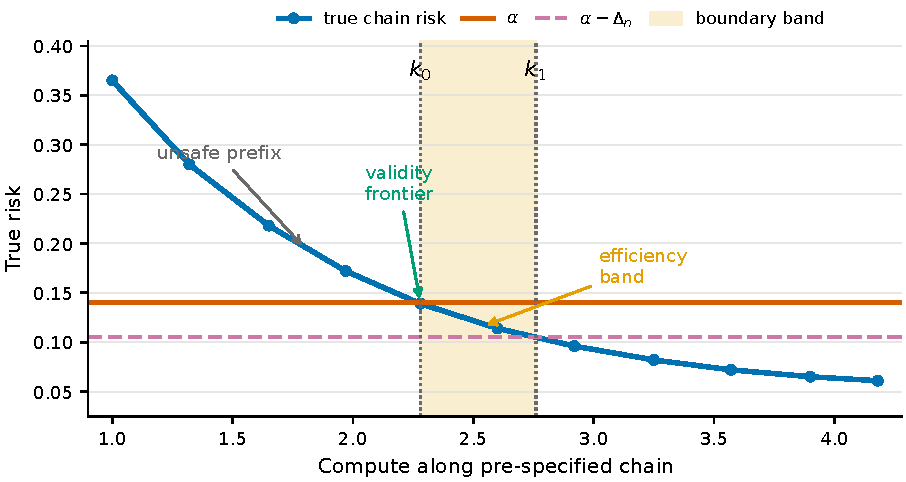
\includegraphics[width=.92\linewidth]{figures/fig2_chain_band.pdf}
\caption{\textbf{Schematic of the compute-chain cost bound.} This is an illustrative monotone-risk chain, not an experimental curve. The fixed-sequence test walks from expensive to cheap. On the validity event, the selected configuration does not undercut the cheapest safe in-chain policy $k_0$. Under Assumption M, the additional compute is bounded by the span between $k_0$ and $k_1$, where $k_1$ is determined by the boundary band $(\alpha-\Delta_n,\alpha]$.}
\label{fig:chain-band}
\end{figure}

\begin{quote}
\textbf{Remark (assumption-free fallback when Assumption M is doubtful).} When per-exit thresholds are tuned jointly, or the empirical-monotonicity diagnostic looks suspect, drop the chain for an FWER procedure that needs no ordering. We implement and evaluate \textbf{Holm's step-down} \cite{holm1979simple}, which is valid unconditionally, requires no monotonicity, and strictly dominates Bonferroni. The general \emph{graphical} family in \cite{bretz2008graphical} subsumes both the chain and Holm and can recycle significance along the compute partial order---reducing to the chain test under exact monotonicity at a $\log|\Lambda|$ band---but we do not implement or evaluate it here, and do not claim its specific behavior.
\end{quote}

\section{Joint risk--compute control}

Problem (P2) additionally certifies a compute budget $B$. The motivation is pre-commitment: an operator who must provision hardware, cap energy, or sign a latency SLA needs the budget guaranteed \emph{before} the test distribution is seen, whereas realized compute can simply be measured afterward. So this is a convenience guarantee layered on the essential risk one, not a co-equal claim. Compute $c_{E_\tau(X)}\in[0,C_{\max}]$ is bounded, so $\hat C(\tau)$ concentrates by Hoeffding: for a single $\tau$, with probability $\ge1-\delta_C$,

\[
C(\tau)\;\le\;\hat C(\tau)+C_{\max}\sqrt{\tfrac{\ln(1/\delta_C)}{2n}}=:U_C(\tau;\delta_C).
\]

To hold uniformly over the data-dependent choice, take a union bound over the $K$ chain points (or $|\Lambda|$ grid points), replacing $\delta_C$ by the \emph{deterministic} $\delta_C/K$ (resp. $\delta_C/|\Lambda|$).

\textbf{Algorithm (dual control).} Split $\delta=\delta_R+\delta_C$. (i) Certify risk: form $\hat\Lambda$ as in Section~3--Section~4 at level $\delta_R$. (ii) Restrict to budget-feasible configs using the \emph{uniform} compute bound: $\hat\Lambda_B=\{\tau\in\hat\Lambda: U_C(\tau;\delta_C/K)\le B\}$. (iii) Output $\hat\tau=\arg\min_{\tau\in\hat\Lambda_B}\hat C(\tau)$, or report infeasible if $\hat\Lambda_B=\varnothing$.

\textbf{Theorem 3 (Joint guarantee).} \emph{With the split budget $\delta=\delta_R+\delta_C$ and the procedure above,}

\[
\Pr\big(R(\hat\tau)\le\alpha \ \text{and}\ C(\hat\tau)\le B\big)\ge1-\delta.
\]

\emph{Proof.} Let $\mathcal A=\{\forall\tau\in\hat\Lambda:R(\tau)\le\alpha\}$ and $\mathcal B=\{\forall\tau\in\Lambda:C(\tau)\le U_C(\tau;\delta_C/K)\}$ (the compute event ranges over the \emph{fixed} grid, with the deterministic correction $\delta_C/K$). By Section~3--Section~4, $\Pr(\mathcal A^c)\le\delta_R$; by Hoeffding and a union bound over the $K$ points, $\Pr(\mathcal B^c)\le\delta_C$. On $\mathcal A\cap\mathcal B$: $\hat\tau\in\hat\Lambda\Rightarrow R(\hat\tau)\le\alpha$, and $\hat\tau\in\hat\Lambda_B\Rightarrow C(\hat\tau)\le U_C(\hat\tau;\delta_C/K)\le B$. Union bound: $\Pr((\mathcal A\cap\mathcal B)^c)\le\delta_R+\delta_C=\delta$. $\square$

A symmetric formulation --- \emph{minimize risk subject to a hard budget} --- swaps the roles, certifying a budget by inverting the compute bound and minimizing $\hat R$ over budget-feasible configs; both are special cases of certifying one functional and optimizing the other.

\textbf{On the split $(\delta_R,\delta_C)$.} We do not present this as a contribution. Because $\delta_R,\delta_C$ enter only through $\sqrt{\ln(1/\cdot)}$, the split is a weak knob: moving mass between the two sides changes each slack only logarithmically. We default to $\delta_R=0.9\delta,\ \delta_C=0.1\delta$ --- favoring the risk side, which is the essential guarantee and whose extra power directly buys cheaper certified policies --- and verify in E5 that performance is flat across a broad central range. An operator who genuinely needs to optimize it faces a trivial one-dimensional search.

\textbf{Looseness of the compute bound.} The range-$C_{\max}$ Hoeffding UCB $U_C$ is conservative, since per-input cost is far from uniform on $[0,C_{\max}]$; in our simulation the dual certificate is reported infeasible whenever the budget $B$ is set near the realized compute, even when a budget-respecting safe policy exists. An empirical-Bernstein compute bound (variance-adaptive, as in Section~6.1) tightens $U_C$ materially and is the recommended form in practice; we keep Hoeffding in the statement for transparency. This is a further reason we treat the compute certificate as secondary to the risk certificate.

\section{Covariate-shift robustness}

Suppose deployment is under $Q$ with $X\sim Q_X$, $Y\mid X$ unchanged, and likelihood ratio $w(x)=\mathrm dQ_X/\mathrm dP_X$. The target is $R_Q(\tau)=\mathbb E_Q[\ell_{\mathrm{loss}}]=\mathbb E_P[w(X)\,\ell_{\mathrm{loss}}]$. The exact-weight case (Section~6.1) is standard; Section~6.2 handles the realistic case where $w$ is estimated.

\subsection{Exact weights (warm-up)}

If $0\le w\le W$ is known exactly, then $w\,\ell_{\mathrm{loss}}\in[0,W]$ has mean $R_Q(\tau)$, and the Section~3.1 argument rescaled by range $W$ gives the valid p-value $p^{Q,\mathrm{exact}}_\tau=\exp(-\frac{2n}{W^2}(\alpha-\hat R_Q(\tau))_+^2)$ with $\hat R_Q(\tau)=\frac1n\sum_i w(X_i)\ell_i$. Theorems 1--2 then hold under $Q$. Two caveats matter in practice. (i) Hoeffding with range $W$ is \emph{loose} for importance weighting because it ignores that most weights are small; the empirical-Bernstein p-value, whose slack scales with the \emph{weighted variance} rather than the range, is materially tighter and is what we use in experiments. (ii) The often-quoted effective sample size $n_{\mathrm{eff}}\approx(\sum_i w_i)^2/\sum_i w_i^2$ describes the behavior of that variance-adaptive bound, \emph{not} of the range-$W$ Hoeffding bound above; we report $n_{\mathrm{eff}}$ only alongside the empirical-Bernstein certificate, to avoid conflating the two.

\subsection{Estimated weights}

Let weights be \textbf{estimated} by any method (density-ratio estimation, a discriminative classifier, moment matching). Two problems arise: (a) the estimator $\hat w$ is a function of data, so treating it as fixed in a Hoeffding bound is invalid; (b) $\hat w\ne w$ introduces bias. We resolve (a) by \textbf{sample splitting} and (b) by an \textbf{$L^1$ error budget}.

Split the calibration set into independent folds $\mathcal D_1$ (size $n_1$) and $\mathcal D_2$ (size $n_2$). Estimate $\hat w$ on $\mathcal D_1$ \emph{only}. Suppose the estimate is bounded, $0\le\hat w\le\hat W$, and obeys an $L^1$ error budget

\begin{equation}
\mathbb E_P\big[\,|\hat w(X)-w(X)|\,\big]\;\le\;\eta
\qquad(\text{conditionally on }\mathcal D_1).
\tag{$\star$}
\end{equation}

Compute the weighted empirical risk on the held-out fold, $\hat R_Q(\tau)=\frac1{n_2}\sum_{i\in\mathcal D_2}\hat w(X_i)\,\ell_i$, and test against the \textbf{deflated} target $\alpha-\eta$:

\begin{equation}
\boxed{\,p^{\,Q}_\tau \;=\; \exp\!\Big(-\tfrac{2 n_2}{\hat W^2}\,\big((\alpha-\eta)-\hat R_Q(\tau)\big)_+^2\Big)\,}.
\tag{3}
\end{equation}

\textbf{Theorem 4 (Shift-robust validity under estimated weights).} \emph{Assume ($\star$), $0\le\hat w\le\hat W$, $\eta<\alpha$, and $Y\mid X$ invariant across $P,Q$. Then the p-value (3) is super-uniform under $H^Q_\tau:R_Q(\tau)>\alpha$, and the chain (or Bonferroni) certification of Section~3--Section~4 applied to $\{p^Q_\tau\}$ at level $\delta$ yields}

\[
\Pr\big(R_Q(\hat\tau)\le\alpha\big)\ge1-\delta\qquad(\text{under }Q).
\]

\emph{Proof.} Condition on $\mathcal D_1$; then $\hat w$ is a fixed (deterministic) function and the summands $\hat w(X_i)\ell_i$ for $i\in\mathcal D_2$ are i.i.d. in $[0,\hat W]$ with common mean $\mu:=\mathbb E_P[\hat w\,\ell_{\mathrm{loss}}]$. Decompose

\[
\mu=\mathbb E_P[w\,\ell_{\mathrm{loss}}]+\mathbb E_P[(\hat w-w)\ell_{\mathrm{loss}}]=R_Q(\tau)+\mathbb E_P[(\hat w-w)\ell_{\mathrm{loss}}].
\]

Since $\ell_{\mathrm{loss}}\in[0,1]$, the bias term is bounded by $|\mathbb E_P[(\hat w-w)\ell_{\mathrm{loss}}]|\le\mathbb E_P|\hat w-w|\le\eta$ by ($\star$). Under $H^Q_\tau$ we have $R_Q(\tau)>\alpha$, hence $\mu\ge R_Q(\tau)-\eta>\alpha-\eta$. By one-sided Hoeffding with range $\hat W$, for any observed $\hat R_Q(\tau)=r\le\alpha-\eta$,

\[
\Pr\big(\hat R_Q(\tau)\le r\,\big|\,\mathcal D_1\big)\le\exp\!\Big(-\tfrac{2n_2}{\hat W^2}(\mu-r)^2\Big)\le\exp\!\Big(-\tfrac{2n_2}{\hat W^2}\big((\alpha-\eta)-r\big)^2\Big)=p^Q_\tau.
\]

So $p^Q_\tau$ is super-uniform under $H^Q_\tau$ conditionally on $\mathcal D_1$; since this holds for every realization of $\mathcal D_1$, it holds marginally. The downstream FWER arguments (Theorems 1--2) are unchanged, run conditionally on $\mathcal D_1$ and then marginalized, giving the stated $1-\delta$ validity under $Q$. $\square$

\textbf{Reading the result.} The three costs are explicit. \emph{(i)} Data splitting shrinks the testing fold to $n_2<n$; we take $n_1$ as small as the weight estimator tolerates, since weight estimation is typically more sample-efficient than the Hoeffding slack on the testing fold. \emph{(ii)} The deflation $\alpha\to\alpha-\eta$ requires $\eta<\alpha$ and makes the certificate conservative in proportion to the weight-error budget. \emph{(iii)} Range inflation $\hat W$ --- mitigated by using the empirical-Bernstein form of (3), exactly as in Section~6.1. The budget $\eta$ has two sources: a theoretical $L^1$ rate for the chosen density-ratio estimator under stated smoothness, or --- more defensibly, since it needs no knowledge of $w$ --- a sensitivity reading: the certificate is valid for any deployment whose weight error is at most $\eta$, so the practitioner reports the largest $\eta^\star$ (the most severe shift) under which the target still holds.

\textbf{Positioning.} The two ingredients are individually standard: conditioning on a held-out fold to make a plug-in estimator a fixed function, and absorbing estimation error into a margin in the spirit of sensitivity analysis (cf. the $\Gamma$-style robustness bounds and estimated-weight treatments in the conformal-under-shift literature \cite{tibshirani2020conformal,jin2023sensitivity}). The contribution is their combination in the LTT risk-control setting, where we have not seen the estimated-weight case stated with a finite-sample proof. We claim validity and interpretability, not tightness.

\textbf{When this is useful, and when it is not.} Two technical limits, both visible in Section~10.1. First, $\eta$ must genuinely upper-bound the estimator's $L^1$ error for validity to hold; it cannot be read off the data. When $\eta$ is set large enough to be defensible, the deflation $\alpha-\eta$ can leave little room and the certificate becomes \emph{infeasible} --- in our simulation feasibility falls toward zero once $\eta$ approaches a fifth of $\alpha$. Thus the result buys robustness at a feasibility price that is acceptable only when the achievable risk sits well below $\alpha$. Second, validity when $\eta$ is \emph{under}-set is not automatic: it held in our simulation only because the fitted density-ratio happened to be conservatively biased; an anti-conservatively biased estimator with $\mathbb E|\hat w-w|>\eta$ can and does breach the target (we exhibit this in Section~10.1 with a deliberately biased estimator). The takeaway is to treat Theorem 4 as a sensitivity statement with a known feasibility cost, not as a general shift solution.

\section{Algorithm summary}

\begin{algorithm}[t]
\caption{Compute-adaptive risk certification}
\begin{algorithmic}[1]
\Require Multi-exit model with exits $1,\ldots,L$; calibration data $\mathcal D$ with $n$ points; target risk $\alpha$; confidence $\delta$; compute-increasing chain $\{\tau^{(1)}\preceq\cdots\preceq\tau^{(K)}=\mathbf 1\}$; optional budget $B$; optional shift inputs $\{\text{weight estimator},\eta\}$; split $(\delta_R,\delta_C)$.
\If{using the shift branch}
  \State Split $\mathcal D$ into $\mathcal D_1,\mathcal D_2$; fit $\hat w$ on $\mathcal D_1$; set the test fold to $\mathcal D_2$, the target to $\alpha-\eta$, and the range to $\hat W$.
\Else
  \State Set the test fold to $\mathcal D$, the target to $\alpha$, and the range to $1$.
\EndIf
\For{each $\tau^{(k)}$}
  \State On the test fold compute $E_{\tau^{(k)}}(X_i)$, predictions, losses $\ell_i$, costs $c_E(X_i)$, empirical risk $\hat R(\tau^{(k)})$ or weighted $\hat R_Q(\tau^{(k)})$, and empirical compute $\hat C(\tau^{(k)})$.
\EndFor
\State Compute p-values $p_k$ using Eq.\ (2), Hoeffding--Bentkus, empirical Bernstein, or weighted Eq.\ (3), at the target and range from step 0.
\State Certify risk with one pre-committed FWER rule: fixed-sequence on the chain, Holm step-down on a finite grid, or Bonferroni on the finite family; call the certified set $\hat\Lambda$.
\If{dual risk--compute control is requested}
  \State Filter $\hat\Lambda_B=\{k\in\hat\Lambda:\hat C(\tau^{(k)})+C_{\max}\sqrt{\ln(K/\delta_C)/(2n_{\mathrm{test}})}\le B\}$.
  \State Output the certified budget-feasible configuration in $\hat\Lambda_B$ with smallest $\hat C$; if none exists, report infeasible.
\Else
  \State Output the certified configuration in $\hat\Lambda$ with smallest $\hat C$; if none exists, report infeasible.
\EndIf
\Ensure The probability of outputting a certified configuration that violates $R(\hat\tau)\le\alpha\ [\text{and } C(\hat\tau)\le B]$ is at most $\delta$, under $Q$ when the shift branch is used and its assumptions hold; an infeasible report carries no risk guarantee.
\end{algorithmic}
\end{algorithm}

Cost: one forward pass collecting all exit scores per calibration point ($O(n)$ inference), then $O(nK)$ to score the chain --- negligible relative to training.

\section{Related work}

\begin{itemize}
\item \textbf{Conformal prediction and risk control.} Split conformal prediction \cite{vovk2022algorithmic,lei2018distributionfree}, conformal risk control \cite{bates2021distributionfree,angelopoulos2024conformal}, and LTT \cite{angelopoulos2025learn} provide distribution-free guarantees for data-dependent prediction-set or model-configuration choices (see \cite{angelopoulos2023gentle} for an introduction). These methods address selection after calibration, whereas naive validation thresholding does not correct for the multiplicity induced by searching over thresholds. Our use of LTT is direct; the added content is the adaptive-inference formulation, the compute-chain efficiency analysis, and the joint risk--compute extension.
\item \textbf{Multiple testing for ordered hypotheses.} Bonferroni, fixed-sequence/fallback procedures \cite{wiens2003fixed}, Holm step-down \cite{holm1979simple}, and graphical sequentially-rejective tests \cite{bretz2008graphical} control family-wise error for finite hypothesis families. These procedures do not by themselves specify which hypothesis order is operationally meaningful for adaptive inference. Here the compute order is fixed before calibration and coincides with the deployment objective: among certified policies, select the cheapest one.
\item \textbf{Adaptive computation.} Surveyed comprehensively in \cite{han2022dynamic,scardapane2020early}, adaptive-depth architectures such as BranchyNet \cite{teerapittayanon2016branchynet}, MSDNet \cite{huang2018multiscale}, SkipNet \cite{wang2018skipnet}, patience-based exiting \cite{zhou2020bert}, and LLM cascades/routers \cite{chen2023frugalgpt} reduce average inference cost by early termination or model routing. Their threshold rules are typically tuned to empirical validation curves, which can produce low compute but does not certify population risk after threshold search. CARC targets this missing calibration layer; it does not alter the backbone architecture.
\item \textbf{Distribution shift.} Weighted conformal prediction \cite{tibshirani2020conformal} and sensitivity-analysis methods for conformal prediction under unknown or misspecified weights \cite{jin2023sensitivity} address deployment distributions different from calibration distributions. Theorem 4 follows the same cautionary pattern: it gives a valid certificate only when the supplied $L^1$ weight-error budget is correct. The result is not a general shift-robust deployment solution; it is a finite-sample sensitivity statement for the LTT risk-control setting.
\item \textbf{Selective prediction.} Selective risk and coverage \cite{geifman2017selective} also formalize when a system may abstain or defer. CARC can encode selective risk through $\ell_{\mathrm{loss}}$, but the primary object here is threshold selection over compute-adaptive policies rather than coverage optimization alone.
\end{itemize}

\begin{table*}[t]
\centering
\caption{Where CARC sits among post-calibration selection methods for adaptive inference. ``DF post-selection risk'': distribution-free risk guarantee for the data-dependent selected policy. ``Compute-ordered search'': the candidate family is tested in an order that coincides with the deployment cost objective. ``Infeasibility reporting'': the procedure explicitly returns ``no certified policy'' rather than a fallback of unknown risk. Entries describe each method's typical native form; weighted or LTT-wrapped variants can extend several rows.}
\label{tab:method-comparison}
\scriptsize
\setlength{\tabcolsep}{6pt}
\begin{tabular}{@{}lccccc@{}}
\toprule
Method & DF post-selection risk & Multiplicity correction & Compute-ordered search & Infeasibility reporting & Covariate-shift certificate \\
\midrule
Naive validation tuning & No & No & Greedy (uncorrected) & No & No \\
Split conformal / conformal risk control \cite{bates2021distributionfree,angelopoulos2024conformal} & Yes & Single parameter & No & Implicit & Weighted variants \\
Learn-then-Test \cite{angelopoulos2025learn} & Yes & Yes (FWER) & Order-agnostic & Implicit & Via weighting \\
CARC (this paper) & Yes & Yes (FWER) & Yes (compute chain) & Yes (explicit) & Yes (sensitivity, Th.~4) \\
\bottomrule
\end{tabular}
\end{table*}

\section{Implementation and evaluation overview}

\textbf{Implemented components.} The implementation follows the theoretical pipeline. A fixed adaptive model first writes cached per-exit scores, predictions, correctness indicators, and cumulative compute. The evaluator converts that cache into loss and cost matrices over a finite threshold chain, computes valid p-values, applies a pre-committed FWER selector, and returns the certified set, selected threshold, feasibility status, and certificate fields for the requested $(\alpha,\delta,B)$. The code implements Hoeffding, Hoeffding--Bentkus, and empirical-Bernstein p-values; Bonferroni, fixed-sequence chain, and Holm selectors; the joint risk--compute test; the estimated-weight shift diagnostic; and cache adapters for synthetic, CIFAR-100 branchy-network, and tabular-cascade settings.

\textbf{Completed evaluations.} The controlled simulation tests the proof-facing properties under oracle risks. The digits tabular-cascade cache tests the same certification path on a feasible real-cache target grid. The CIFAR-100 branchy-cache run tests the failure mode in which the trained model cannot meet most preregistered targets and the correct output is usually infeasibility. Wall-clock latency and hardware-dependent throughput are not certified quantities in this manuscript; compute is represented by the pre-specified cost proxy in each cache.

\section{Experiments}

The experiments follow the pipeline induced by the theory. First, the controlled simulation verifies finite-sample validity and compute behavior in a setting where true risk is known. Second, the digits real-cache experiment evaluates the same certification path when the target grid is feasible before calibration. Third, the CIFAR-100 branchy-cache experiment evaluates the opposite case, where most preregistered targets are below the finite-pool risk frontier and the correct certified outcome is usually infeasibility. Larger vision, language, and real-shift deployments remain outside the evidence base of this manuscript.

Figure~\ref{fig:empirical-summary} summarizes the controlled simulation, CIFAR diagnostic, and synthetic shift sensitivity sweep. Table~\ref{tab:digits-confirmatory} reports the positive real-cache validation. These artifacts should be read as scoped evidence: simulation verifies theorem-level behavior with oracle risks; digits validates the cache evaluator on a feasible real-cache grid; CIFAR diagnoses infeasibility for a particular branchy model and target grid; and the shift experiment is a sensitivity analysis rather than a general shift-robust deployment claim.

\begin{figure}[t]
\centering
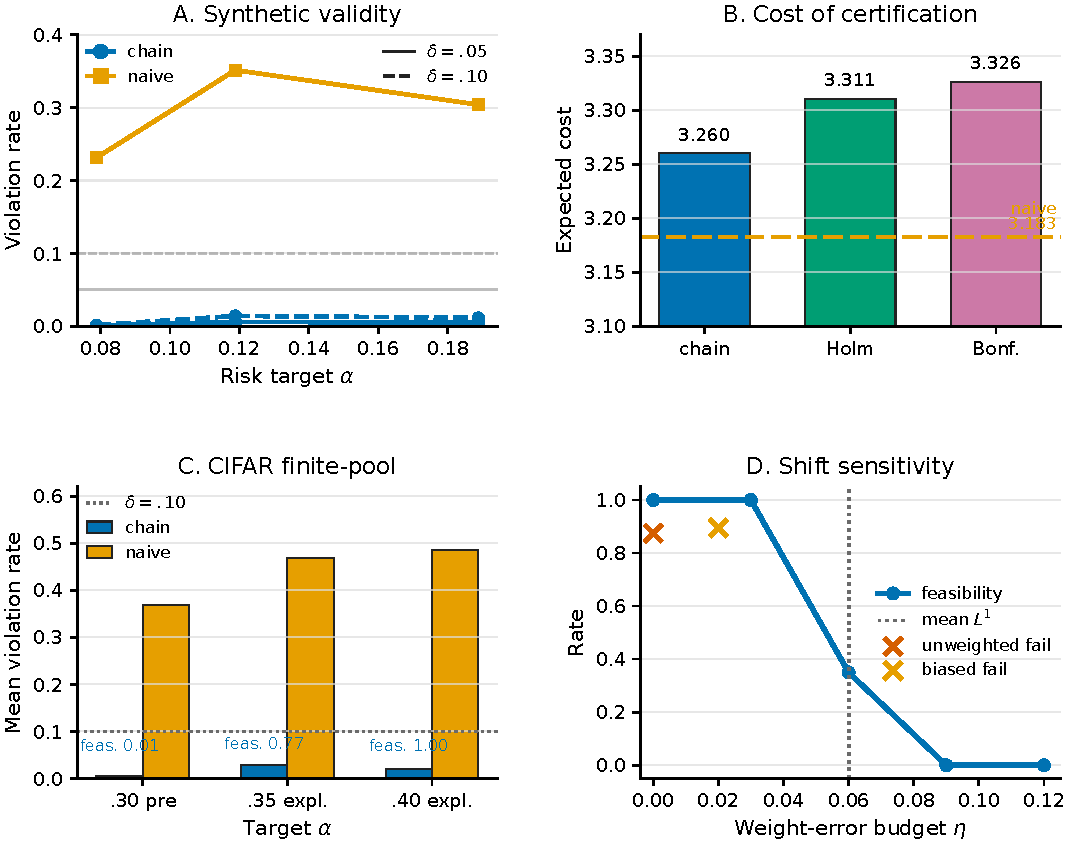
\includegraphics[width=\linewidth]{figures/fig3_empirical_summary.pdf}
\caption{\textbf{Empirical evidence summary from the completed studies.} (A) In the controlled simulation, the certified chain stays below the nominal violation levels while naive validation inspection violates far above them. (B) In the representative E2 cell, the chain has lower certified expected cost than Holm or Bonferroni, and remains close to the invalid naive reference. (C) In the CIFAR-100 finite-pool diagnostic, bars show mean violation rates across the reported split cells for each target and method; vertical labels give mean feasibility, and exact cell values are in Tables~\ref{tab:embedded-cifar-preregistered}--\ref{tab:embedded-cifar-exploratory}. The $\alpha=0.30$ target is pre-registered but infeasible in full-pool risk; $\alpha\in\{0.35,0.40\}$ is exploratory. (D) Under shift, an undersized or biased weight budget can fail, while defensible $\eta$ values make the estimated-weight certificate infeasible in this synthetic sweep.}
\label{fig:empirical-summary}
\end{figure}

\subsection{Controlled-simulation verification}

We use a synthetic early-exit model ($L=5$ exits, competence increasing with depth, noisy confidences, global-threshold chain of $K=40$ configurations) whose true per-configuration risk and cost are computable by large-sample Monte Carlo. This setting isolates the statistical guarantee: every selected policy can be checked against true risk rather than a held-out finite-pool proxy. It is not evidence about real network accuracy or hardware performance, and it does not validate Assumption M or weight estimability in deployment. The complete row-level numerical outputs are embedded in Tables~\ref{tab:embedded-e1}--\ref{tab:embedded-e6}.

\emph{Validity and naive failure (E1/E3).} Across a grid of targets and $T=3000$ calibration/test splits per cell, the certified chain violates $R(\hat\tau)\le\alpha$ at rates of $0.0010$--$0.0143$, all below $\delta\in\{0.05,0.10\}$. The naive recipe (cheapest configuration with $\hat R\le\alpha$, no multiplicity correction) violates at $0.2313$--$0.3513$. Thus, in the oracle-risk simulation, post-selection calibration error is not a small perturbation; it is the dominant failure mode of the uncorrected baseline.

\emph{Cost of the guarantee (E2).} At a representative $(\alpha,\delta)=(0.119,0.10)$ with $T=2000$, the certified expected cost is $3.260$ for the chain, $3.311$ for Holm, and $3.326$ for Bonferroni; all three certified selectors satisfy the tested violation constraint. At the matched E1 target, the invalid naive policy costs $3.183$. The chain therefore pays a small premium over the invalid baseline in this synthetic setting, and its advantage over Bonferroni is modest. The result supports the theoretical distinction between validity and efficiency, but it does not imply that the compute premium will be small for every trained model or target.

\emph{Joint control (E5).} With $\alpha=0.089$, $\delta=0.10$, $n=2000$, and $T=1000$, a slack budget $B=4.641$ is certified feasible in every trial, with no true risk violations and mean certified compute UCB $3.620$. A tight budget $B=3.363$ is oracle-feasible --- the cheapest truly safe configuration costs $3.313$ --- but the range-$C_{\max}$ compute certificate reports infeasible in every trial. This quantifies the conservativeness flagged in Section~5.

\emph{Covariate shift (E6).} Under an exp-tilt shift toward harder inputs, the unweighted source-calibrated certificate violates the target at rate $0.875$. The estimated-weight sweep has realized mean weight error $\|\hat w-w\|_1\approx0.060$: when $\eta\in\{0,0.03\}$, the certificate remains feasible with $0$ observed violations but lacks the assumption required by Theorem 4; at $\eta=0.06$, feasibility drops to $0.35$; and at $\eta\in\{0.09,0.12\}$, feasibility is $0$. With a deliberately downward-biased estimator and an underspecified $\eta=0.02$ ($\|\hat w-w\|_1\approx0.351$), the certificate violates at rate $0.895\gg\delta$. These results calibrate Theorem 4 as a sensitivity tool, not as a robustification method that can be applied without a defensible weight-error budget.

\subsection{Digits tabular-cascade real-cache confirmation}

The confirmatory real-cache study uses the scikit-learn digits data with a three-exit tabular cascade: Gaussian naive Bayes, logistic regression, and support-vector classification, with relative exit costs $1.0$, $4.0$, and $12.0$. The train/cache split is fixed by seed $20260615$; the cache contains $899$ examples, $64$ features, and $10$ classes. The full-pool exit accuracies are $0.863$, $0.968$, and $0.981$, and the final-exit full-pool risk is $0.0189$. Thus the preregistered targets $\alpha\in\{0.05,0.10,0.15\}$ are feasible before calibration. The grid uses Hoeffding--Bentkus p-values, $T=1000$ calibration/test partitions per cell, $\delta\in\{0.05,0.10\}$, and calibration sizes $\{100,300\}$. Violation rates are counted over all split attempts; infeasible reports count as no certified violation but are exposed through the feasibility column.

Across all 12 chain cells, the empirical violation rate is $0$--$0.051$, and no cell exceeds its matching $\delta$. The most informative contrast is at $\alpha=0.10$: the chain selects in $0.884$--$1.000$ of trials, violates at $0.002$--$0.018$, and has mean cost $11.800$--$11.979$; naive validation inspection violates at $0.486$--$0.571$ while spending $5.14$--$6.09$ fewer relative cost units. At $\alpha=0.05$, the stringent target often forces the final exit. At $\alpha=0.15$, the target is easier and the naive baseline can be safe in some cells, but Table~\ref{tab:digits-confirmatory} still reports the compute premium of certification. This experiment is not a claim about tabular classification performance; it validates that the cache-based CARC pipeline reports feasible targets, infeasibility, violation rates, and compute premium without tuning on test splits. The cascade is intentionally non-neural: it isolates the calibration layer, which depends on the trained system only through the cached scores, losses, and costs, and is therefore exercised faithfully here even though the backbone is not a deep early-exit network.

\begin{table*}[t]
\centering
\caption{Preregistered digits tabular-cascade real-cache confirmation. The cache uses $899$ examples, $K=101$ scalar thresholds, Hoeffding--Bentkus p-values, $T=1000$, violation denominator ``all'', and relative costs $[1,4,12]$. The certified compute premium is mean chain cost minus mean naive cost in the same relative cost units.}
\label{tab:digits-confirmatory}
\scriptsize
\setlength{\tabcolsep}{4pt}
\begin{tabular}{@{}cccccccc@{}}
\toprule
$\alpha$ & $\delta$ & $n_{\mathrm{cal}}$ & Chain feas. & Chain viol. & 95\% CI & Chain cost & Naive viol. / premium \\
\midrule
0.05 & 0.05 & 100 & 0.139 & 0.000 & [0.000,0.004] & 12.000 & 0.045 / 0.483 \\
0.05 & 0.05 & 300 & 0.832 & 0.000 & [0.000,0.004] & 12.000 & 0.000 / 0.000 \\
0.05 & 0.10 & 100 & 0.413 & 0.000 & [0.000,0.004] & 12.000 & 0.047 / 0.503 \\
0.05 & 0.10 & 300 & 0.924 & 0.000 & [0.000,0.004] & 12.000 & 0.000 / 0.000 \\
0.10 & 0.05 & 100 & 0.884 & 0.007 & [0.003,0.014] & 11.915 & 0.571 / 6.092 \\
0.10 & 0.05 & 300 & 1.000 & 0.002 & [0.000,0.007] & 11.979 & 0.497 / 5.281 \\
0.10 & 0.10 & 100 & 0.964 & 0.018 & [0.011,0.028] & 11.800 & 0.522 / 5.444 \\
0.10 & 0.10 & 300 & 1.000 & 0.004 & [0.001,0.010] & 11.958 & 0.486 / 5.142 \\
0.15 & 0.05 & 100 & 1.000 & 0.000 & [0.000,0.004] & 10.115 & 0.000 / 8.701 \\
0.15 & 0.05 & 300 & 1.000 & 0.034 & [0.024,0.047] & 4.985 & 0.049 / 3.971 \\
0.15 & 0.10 & 100 & 1.000 & 0.001 & [0.000,0.006] & 8.803 & 0.001 / 7.330 \\
0.15 & 0.10 & 300 & 1.000 & 0.051 & [0.038,0.067] & 4.049 & 0.051 / 3.024 \\
\bottomrule
\end{tabular}
\end{table*}

\subsection{CIFAR-100 real-cache diagnostic}

The CIFAR-100 study is a deliberate stress test of the most safety-critical behavior in CARC: what the procedure does when the trained system cannot meet the requested targets. The correct response is to certify nothing and report infeasibility, and the value of that response is measured against what an uncorrected baseline would have deployed in its place. The diagnostic uses a branchy ResNet-56-style model with four exits (after the stem and after each of three residual stages), scalar top-softmax thresholds on a $K=100$ grid, 0--1 loss, and analytical cumulative MAC estimates. The model was trained for 80 epochs and evaluated on the CIFAR-100 test set. The per-exit test accuracies are $0.0646$, $0.3040$, $0.6147$, and $0.6945$; the corresponding cumulative exit costs are $0.44$, $42.91$, $84.33$, and $125.75$ million MACs. Because this is a finite test-pool diagnostic, the reported violation frequencies use held-out split risk as a proxy for population risk, not as an oracle truth measurement. The complete row-level numerical outputs are embedded in Tables~\ref{tab:embedded-cifar-preregistered}--\ref{tab:embedded-cifar-exploratory}.

\textbf{Pre-registered CIFAR grid.} The frozen CIFAR E1 grid uses $\alpha\in\{0.05,0.10,0.20,0.30\}$, $\delta\in\{0.05,0.10\}$, calibration sizes $\{500,2000\}$, Hoeffding--Bentkus p-values, and $T=1000$ random calibration/test partitions per cell. The full test-pool minimum risk along the chain is $0.3055$, so none of the pre-registered targets has a truly safe configuration. The certified chain therefore mostly reports infeasibility. Its violation frequency over all split attempts is $0$ for $\alpha\le0.20$ and $0.000$--$0.013$ at $\alpha=0.30$, but feasibility at $\alpha=0.30$ is only $0.000$--$0.013$. The naive selector instead selects in $0.281$--$0.457$ of the $\alpha=0.30$ split attempts and violates in exactly those attempts, because the selected finite-pool policies remain above the target. This result supports the infeasibility-reporting behavior and exposes the naive failure mode; it does not support a claim that this CIFAR model enables low-error certified deployment at the preregistered targets.

\textbf{Exploratory feasible-target check.} To confirm that the cache evaluator behaves sensibly once the target is feasible, we ran a post hoc diagnostic at $\alpha\in\{0.35,0.40\}$ with the same $\delta$, calibration sizes, p-values, and split count. The chain violation frequencies are $0.012$--$0.038$, always below the corresponding $\delta$; naive validation tuning violates at $0.441$--$0.529$. Chain feasibility is high for $\alpha=0.40$ ($0.994$--$1.000$) and mixed for $\alpha=0.35$ ($0.484$--$0.996$), matching the fact that the feasible frontier is close to the final-exit risk. Mean chain cost is $85.65$--$105.30$ million MACs across these feasible-target cells, compared with $81.28$--$92.85$ million MACs for the invalid naive policy. Holm and Bonferroni are more conservative: they have lower or zero violation rates but lower feasibility and higher mean cost in the same cells.

\textbf{Monotonicity diagnostic.} The full-pool chain risk is not perfectly nonincreasing: four adjacent threshold pairs show risk increases, with maximum increase $2\times10^{-4}$, while cost is nondecreasing. This small empirical violation does not affect validity, but it means the Assumption M efficiency interpretation should be read as a diagnostic rather than a confirmed model property on this cache.

\section{Limitations}

\begin{itemize}
\item \textbf{Calibration assumptions.} The base validity result assumes i.i.d. calibration data from the deployment distribution. Under covariate shift, Theorem 4 additionally requires an $L^1$ weight-error budget $\eta$; if the budget is incorrect or the shift is unmodeled, the certificate can fail.
\item \textbf{Loss assumptions.} The concentration bounds require bounded losses. Unbounded or heavy-tailed risk functionals require different concentration arguments, such as truncation or variance-adaptive bounds with additional conditions.
\item \textbf{Search scope.} Cost-optimality is only within the chosen finite chain. A scalar threshold chain is a one-dimensional subset of the full per-exit threshold space, and neither the chain nor the implemented Holm baseline exhausts the continuum of possible policies.
\item \textbf{Compute model.} The certified compute functional uses the pre-specified cost proxy $c_\ell$. In the CIFAR diagnostic this proxy is analytical MAC count, not measured wall-clock latency. Hardware latency under batching, memory effects, and accelerator scheduling must be evaluated separately before deployment.
\item \textbf{Efficiency assumptions.} Assumption M affects the efficiency interpretation, not validity. If risk is not monotone along the compute chain, the selector remains protected by FWER control, but the chain-order cost bound should not be read as an empirical efficiency guarantee. The reported monotonicity diagnostic is necessary but not sufficient for the true-risk condition.
\item \textbf{Empirical scope.} The real-cache evidence consists of a feasible digits cascade and a CIFAR-100 diagnostic on a modest branchy CNN. This is not a comprehensive benchmark suite. The CIFAR preregistered target grid is mostly infeasible because the final-exit test risk is $0.3055$, and the feasible CIFAR targets are exploratory.
\item \textbf{Shift certificate.} Theorem 4 is a conservative sufficient condition. When $\eta$ is large enough to be defensible, the deflated target can make certification infeasible; when $\eta$ is too small, the target can be breached. The budget must therefore come from an external estimator guarantee or be reported as a sensitivity parameter.
\item \textbf{Single-use protocol.} The guarantee is for one pre-specified run of the procedure. Sweeping multiple $(\alpha,\delta,\text{chain})$ choices on the same calibration set and then selecting the most favorable outcome reintroduces multiplicity outside the stated guarantee.
\item \textbf{Future validation.} The next empirical step is not additional tuning on the present caches; it is preregistered evaluation on larger early-exit models, language-model cascades, measured hardware latency, and non-synthetic distribution shifts, with infeasibility and compute premium reported alongside violation rates.
\end{itemize}

\section{Engineering and deployment considerations}

The intended deployment role of CARC is narrow: it is a calibration layer for a fixed adaptive inference system. It can certify a threshold policy, report that no candidate certifies, or quantify the compute premium of certification relative to an uncorrected baseline. It does not improve the trained model, repair poor final-exit accuracy, or guarantee latency under hardware effects not represented in $c_\ell$. The main operational risk is over-trust: an infeasible report, a finite-pool diagnostic, or an exploratory feasible-target check can be mistaken for a population-level deployment guarantee. The manuscript mitigates this risk by stating assumptions at the point of use, separating feasibility from validity, and requiring $(\alpha,\delta)$, the chain, and the split protocol to be fixed before calibration risks are inspected.

\textbf{A worked deployment read.} Table~\ref{tab:digits-confirmatory} can be read as an operator would use it. Suppose the target is at most $10\%$ error with $95\%$ confidence ($\alpha=0.10$, $\delta=0.05$) and $300$ calibration points are available. CARC certifies a policy in every trial at mean relative cost $11.98$ while violating the target in only $0.2\%$ of calibration draws; the uncorrected baseline is about $5.3$ cost units cheaper but violates the $10\%$ target in roughly half of the draws---that gap is the price of the guarantee. Tightening the target to $\alpha=0.05$ with only $100$ calibration points instead gives feasibility $0.139$: CARC usually reports infeasibility, correctly signaling that this system, at this calibration size, cannot certify $5\%$ error and that the operator should collect more data, relax the target, or improve the model rather than deploy on faith. Relaxing the target to $\alpha=0.15$ moves the certified policy to a much cheaper exit (mean cost $4.05$), so the certified operating point tracks the requested risk level.

\section{Conclusion}

This paper formulates threshold selection for compute-adaptive inference as finite-family risk control. By instantiating LTT on a compute-ordered candidate chain, CARC separates three quantities that are often conflated in validation tuning: risk validity, feasibility of the target for the trained system, and compute efficiency of the certified policy. The theory proves distribution-free validity for certified selectors, characterizes the finite-sample compute band of the fixed-sequence chain under monotone risk, adds a conservative joint risk--compute certificate, and gives an estimated-weight sufficient condition for covariate shift.

The empirical results support these claims within their stated scope. In simulation with oracle risks, certified selection respects the tested violation levels while naive validation thresholding violates substantially. On the preregistered digits cache, the certificate remains within the tested violation levels on a feasible target grid, whereas naive tuning fails sharply at $\alpha=0.10$. On CIFAR-100, the preregistered target grid is mostly infeasible; the correct interpretation is that the trained branchy model does not support those certified risk targets, not that CARC fails to find a hidden low-risk policy. The main limitation is empirical breadth: larger early-exit networks, language cascades, measured latency, and non-synthetic shift studies remain to be evaluated under the same preregistered protocol. Future work should also replace the conservative range-based compute bound with tighter variance-adaptive or hardware-aware certificates while preserving finite-sample validity.

\section{Data and code availability}

The current reference implementation covers the p-values, certification procedures, selectors, controlled-simulation scripts, CIFAR cache adapter, tabular-cascade adapter, and cache-based real-data evaluator. The digits real-cache result is summarized in Table~\ref{tab:digits-confirmatory}; the synthetic and CIFAR row-level results are embedded in Appendix~B. The corresponding JSON artifacts are \texttt{results/digits\_tabular\_real\_cache\_eval.json}, \texttt{results/cifar\_branchy\_real\_cache\_eval.json}, and \texttt{results/cifar\_branchy\_real\_cache\_eval\_exploratory.json}. All $(\alpha,\delta,B)$ grids, seeds, split counts, and pass criteria used for reported experiments are specified in the source files or in \texttt{preregistration.md}; exploratory CIFAR cells are labeled separately. The source repository and archival DOI should be inserted here before IEEE Access submission.

\section*{Acknowledgment}

Author acknowledgments, funding information, and any required disclosure about AI-assisted text generation are to be completed before IEEE Access submission.

\onecolumn
\appendix

\section{Proofs}

Throughout, losses are in $[0,1]$, calibration data are $n$ i.i.d. draws from $P$, and $\epsilon_n(\beta):=\sqrt{\ln(1/\beta)/(2n)}$. A p-value $p$ for a null $H$ is \emph{valid} (super-uniform) if $\Pr_H(p\le u)\le u$ for all $u\in(0,1)$.

\subsection{Validity of the Hoeffding p-value (Eq. 2)}

\emph{Claim.} $p_\tau=\exp(-2n(\alpha-\hat R(\tau))_+^2)$ is valid for the null $H_\tau:R(\tau)>\alpha$ of Section~3; super-uniformity is established over its closure $R(\tau)\ge\alpha$, the supremum of the rejection probability being attained at the boundary $R(\tau)=\alpha$.

\emph{Proof.} Fix $\tau$ and write $R=R(\tau)$, $\hat R=\hat R(\tau)$. For $u\in(0,1)$, $p_\tau\le u \iff (\alpha-\hat R)_+\ge\epsilon_n(u) \iff \hat R\le\alpha-\epsilon_n(u)$ (the event is empty if $\alpha-\epsilon_n(u)<0$, making the probability $0\le u$ trivially). Under $H_\tau$, $R\ge\alpha$, so

\[
\Pr_{H_\tau}(p_\tau\le u)=\Pr(\hat R\le\alpha-\epsilon_n(u))\le\Pr(\hat R\le R-\epsilon_n(u))\le e^{-2n\epsilon_n(u)^2}=u,
\]

where the second inequality uses $\alpha\le R$ and the third is the lower-tail Hoeffding inequality for the mean of $n$ i.i.d. $[0,1]$ variables. Hence $p_\tau$ is super-uniform. The supremum over the composite null is attained at the boundary $R=\alpha$, as used above. $\square$

\subsection{Bonferroni FWER (Theorem 1)}

\emph{Claim.} With $\hat\Lambda_{\mathrm{Bonf}}=\{\tau:p_\tau\le\delta/|\Lambda|\}$ and valid $\{p_\tau\}$, $\Pr(\exists\tau\in\hat\Lambda_{\mathrm{Bonf}}:R(\tau)>\alpha)\le\delta$.

\emph{Proof.} Let $\mathcal N=\{\tau:R(\tau)>\alpha\}$ be the true nulls. The bad event is $\bigcup_{\tau\in\mathcal N}\{p_\tau\le\delta/|\Lambda|\}$. By validity, $\Pr(p_\tau\le\delta/|\Lambda|)\le\delta/|\Lambda|$ for each $\tau\in\mathcal N$, so by the union bound the probability is at most $|\mathcal N|\cdot\delta/|\Lambda|\le|\Lambda|\cdot\delta/|\Lambda|=\delta$. Restricting any selection rule to the complement of the bad event yields a safe certified output. If the certified set is empty, the procedure reports infeasibility and makes no certified-risk claim about any operational fallback. $\square$

\subsection{Fixed-sequence FWER (Theorem 2(a))}

\emph{Claim.} Testing a pre-specified order $\tau^{(K)},\dots,\tau^{(1)}$, certifying while $p_{\tau^{(k)}}\le\delta$ and stopping at the first failure, controls the probability of certifying any unsafe configuration at $\delta$, independent of $K$.

\emph{Proof.} Let $j^\star$ be the position of the first true null in the testing order (the first tested $\tau^{(k)}$ with $R(\tau^{(k)})>\alpha$); if there is none, no unsafe config exists and the error probability is $0$. The procedure certifies a configuration only if it certifies everything earlier in the order, so it certifies an unsafe configuration only if it certifies the one at position $j^\star$ --- which requires $p$ at that position $\le\delta$. Because the order is fixed \emph{before} seeing the data, that hypothesis is a fixed true null, and by validity $\Pr(p\le\delta)\le\delta$. Thus the probability of certifying any unsafe configuration is at most $\delta$, with no dependence on $K$ (no correction is applied). $\square$

\subsection{Two-sided cost bound (Theorem 2(b))}

Stated and proved in full in the dedicated subsection below (kept separate for length). It establishes $\Pr(k_0\le k^\star\le k_1)\ge1-2\delta$ with band $\Delta_n=\epsilon_n(\delta)+\epsilon_n(\delta/K)$, so validity carries no $K$-penalty while the search cost is an $O(\sqrt{\ln(K/\delta)/n})$ efficiency band.

\subsection{Joint risk--compute control (Theorem 3)}

\emph{Claim.} With $\delta=\delta_R+\delta_C$, risk certified at $\delta_R$ (Section~A.2--A.4) and the uniform compute bound $U_C(\tau;\delta_C/K)=\hat C(\tau)+C_{\max}\sqrt{\ln(K/\delta_C)/(2n)}$ over the $K$ chain points, the probability that the dual selector outputs a configuration violating either $R(\hat\tau)\le\alpha$ or $C(\hat\tau)\le B$ is at most $\delta$. If the budget-certified set is empty, the selector reports infeasibility.

\emph{Proof.} Define $\mathcal A=\{\forall\tau\in\hat\Lambda:R(\tau)\le\alpha\}$ (the risk-certification event) and $\mathcal B=\{\forall k:C(\tau^{(k)})\le U_C(\tau^{(k)};\delta_C/K)\}$. For $\mathcal B$: $c_{E_\tau(X)}\in[0,C_{\max}]$, so for each fixed $k$, upper-tail Hoeffding gives $\Pr(C(\tau^{(k)})>U_C(\tau^{(k)};\delta_C/K))\le\delta_C/K$; a union bound over the $K$ (data-independent) points gives $\Pr(\mathcal B^c)\le\delta_C$. By construction $\Pr(\mathcal A^c)\le\delta_R$. On $\mathcal A\cap\mathcal B$, the selected $\hat\tau\in\hat\Lambda$ has $R(\hat\tau)\le\alpha$, and $\hat\tau\in\hat\Lambda_B$ forces $C(\hat\tau)\le U_C(\hat\tau;\delta_C/K)\le B$. Boole: $\Pr((\mathcal A\cap\mathcal B)^c)\le\delta_R+\delta_C=\delta$. The denominator $K$ is deterministic, so no data-dependent correction is involved. $\square$

\subsection{Estimated-weight shift certificate (Theorem 4)}

\emph{Claim.} Under ($\star$) $\mathbb E_P|\hat w-w|\le\eta$ (conditionally on $\mathcal D_1$), $0\le\hat w\le\hat W$, $\eta<\alpha$, and $Y\mid X$ invariant, the p-value (3) is valid for $H^Q_\tau:R_Q(\tau)>\alpha$, and certification at level $\delta$ gives $\Pr(R_Q(\hat\tau)\le\alpha)\ge1-\delta$ under $Q$.

\emph{Proof.} Condition on $\mathcal D_1$. Then $\hat w$ is a fixed measurable function, and for $i\in\mathcal D_2$ the variables $\hat w(X_i)\ell_i$ are i.i.d. on $[0,\hat W]$ with common mean $\mu:=\mathbb E_P[\hat w\,\ell_{\mathrm{loss}}]$. Decompose $\mu=R_Q(\tau)+\mathbb E_P[(\hat w-w)\ell_{\mathrm{loss}}]$, using $R_Q(\tau)=\mathbb E_P[w\,\ell_{\mathrm{loss}}]$ (which holds because $Y\mid X$ is invariant). Since $\ell_{\mathrm{loss}}\in[0,1]$, the bias term is bounded: $|\mathbb E_P[(\hat w-w)\ell_{\mathrm{loss}}]|\le\mathbb E_P|\hat w-w|\le\eta$. Under $H^Q_\tau$, $R_Q(\tau)>\alpha$, hence $\mu>\alpha-\eta$. For observed $\hat R_Q=r\le\alpha-\eta$, the range-$\hat W$ Hoeffding inequality gives

\[
\Pr(\hat R_Q\le r\mid\mathcal D_1)\le\exp\!\Big(-\tfrac{2n_2}{\hat W^2}(\mu-r)^2\Big)\le\exp\!\Big(-\tfrac{2n_2}{\hat W^2}((\alpha-\eta)-r)^2\Big)=p^Q_\tau.
\]

So $p^Q_\tau$ is super-uniform under $H^Q_\tau$ conditionally on $\mathcal D_1$; since this holds for every realization of $\mathcal D_1$, it holds marginally (integrate over $\mathcal D_1$). The FWER arguments of A.2--A.4 then run conditionally on $\mathcal D_1$ and marginalize, giving $1-\delta$ validity under $Q$. The empirical-Bernstein variant replaces the range-$\hat W$ Hoeffding step with A.7 applied on $[0,\hat W]$, unchanged otherwise. $\square$

\subsection{Hoeffding--Bentkus and empirical-Bernstein p-values}

\textbf{Hoeffding--Bentkus.} For $H:R\ge\alpha$ with $\hat R$ the mean of $n$ i.i.d. $[0,1]$ losses, the p-value $p^{\mathrm{HB}}=\min\{\exp(-n\,\mathrm{kl}(\hat R,\alpha)),\ e\,\Pr(\mathrm{Bin}(n,\alpha)\le\lceil n\hat R\rceil)\}$ (with $\mathrm{kl}$ the binary KL divergence, and $p^{\mathrm{HB}}=1$ if $\hat R\ge\alpha$) is valid; the first term is the Cram{\'e}r--Chernoff (relative-entropy) bound and the second the Bentkus inequality, each super-uniform under $H$, so their minimum is super-uniform. We use this as the default in experiments and rely on the concentration inequalities used in \cite{bates2021distributionfree}, \cite{angelopoulos2025learn}, and \cite{angelopoulos2024conformal}, together with Bentkus's bound \cite{bentkus2004hoeffding}.

\textbf{Empirical Bernstein (as implemented).} Let $\hat V_n$ be the unbiased sample variance of the $n$ losses (range $\rho$; $\rho=1$ unweighted, $\rho=\hat W$ weighted). The one-sided empirical-Bernstein inequality in \cite{maurer2009empirical} states that, for every $\beta\in(0,1)$,

\begin{equation}
\Pr\Big(R-\hat R\ \ge\ \sqrt{\tfrac{2\hat V_n\ln(1/\beta)}{n}}+\tfrac{7\rho\ln(1/\beta)}{3(n-1)}\Big)\ \le\ \beta. \tag{MP}
\end{equation}

Define, for observed $(\hat R,\hat V_n)$ with $\hat R<\alpha$, the value $u^\star\ge0$ solving

\[
\alpha-\hat R\ =\ \sqrt{\tfrac{2\hat V_n}{n}}\,\sqrt{u^\star}\ +\ \tfrac{7\rho}{3(n-1)}\,u^\star
\]

(the right side is continuous and strictly increasing from $0$ to $\infty$ in $u^\star$, so the root is unique; in closed form, with $a=\sqrt{2\hat V_n/n}$, $b=7\rho/(3(n-1))$, $c=\alpha-\hat R$, $\sqrt{u^\star}=(-a+\sqrt{a^2+4bc})/(2b)$). Set $p^{\mathrm{EB}}=\exp(-u^\star)$ (and $p^{\mathrm{EB}}=1$ if $\hat R\ge\alpha$).

\emph{Claim.} $p^{\mathrm{EB}}$ is valid for $H:R\ge\alpha$.

\emph{Proof.} Because the deviation $D(\beta):=\sqrt{2\hat V_n\ln(1/\beta)/n}+7\rho\ln(1/\beta)/(3(n-1))$ is strictly increasing in $\ln(1/\beta)$, the definition of $u^\star$ gives the equivalence $p^{\mathrm{EB}}\le\beta\iff u^\star\ge\ln(1/\beta)\iff \alpha-\hat R\ge D(\beta)$. Under $H$, $R\ge\alpha$, so $\{\alpha-\hat R\ge D(\beta)\}\subseteq\{R-\hat R\ge D(\beta)\}$, and by (MP),

\[
\Pr_H(p^{\mathrm{EB}}\le\beta)=\Pr_H(\alpha-\hat R\ge D(\beta))\le\Pr_H(R-\hat R\ge D(\beta))\le\beta.
\]

Hence $p^{\mathrm{EB}}$ is super-uniform. Validity holds with $\hat V_n$ random because (MP) is itself an empirical-variance inequality, valid simultaneously over the realized $\hat V_n$. $\square$

(The reference implementation computes exactly this $u^\star$; the unit tests confirm $\Pr(p\le\beta)\le\beta$ under $R=\alpha$ by Monte Carlo for all three p-values.)

\subsection{Full proof of the two-sided cost bound (Theorem 2(b))}

\textbf{Standing notation.}

(N1) Calibration data $\mathcal D=\{(X_i,Y_i)\}_{i=1}^n$ i.i.d. from $P$.

(N2) Chain $\tau^{(1)},\dots,\tau^{(K)}$ with deterministically nondecreasing compute $C_1\le\dots\le C_K$, where $C_k:=C(\tau^{(k)})$ (Section~4.1: raising the global threshold can only push each input to a deeper exit, so the per-input cost $c_{E_{\tau^{(k)}}(\cdot)}$ is pointwise nondecreasing in $k$, hence so is its expectation).

(N3) Per-point losses $\ell_{ik}:=\ell_{\mathrm{loss}}(\hat Y_{\tau^{(k)}}(X_i),Y_i)\in[0,1]$; $\hat R_k:=\frac1n\sum_i\ell_{ik}$, $R_k:=\mathbb E[\hat R_k]=R(\tau^{(k)})$.

(N4) Slack $\epsilon_n(\beta):=\sqrt{\ln(1/\beta)/(2n)}$. With the Hoeffding p-value $p_k=\exp(-2n(\alpha-\hat R_k)_+^2)$, the certification test $p_k\le\delta$ is \textbf{exactly} $\hat R_k\le\alpha-\epsilon_n(\delta)$.

The fixed-sequence walk from expensive to cheap certifies a suffix of the compute order; equivalently

\[
k^\star\;=\;\min\Big\{\,k:\ \hat R_j\le\alpha-\epsilon_n(\delta)\ \text{for all}\ j\ge k\,\Big\},
\]

with the convention $k^\star:=K+1$ (report infeasible) if the set is empty. Output $\hat\tau=\tau^{(k^\star)}$ only when $k^\star\le K$. For cost-accounting diagnostics one may record $\tau^{(K)}$ as an operational fallback in infeasible cells, but that fallback is not a certified output unless it separately certifies. Let $k_0:=\min\{k:R_k\le\alpha\}$ be the cheapest truly-safe index ($k_0:=K+1$ if no config is safe).

\textbf{Lemma A.4.1 (Hoeffding, both tails).} For each fixed $k$ and any $t\ge0$,

\[
\Pr(\hat R_k\le R_k-t)\le e^{-2nt^2},\qquad \Pr(\hat R_k\ge R_k+t)\le e^{-2nt^2}.
\]

\emph{Proof.} The $\{\ell_{ik}\}_{i=1}^n$ are i.i.d. in $[0,1]$ with mean $R_k$; apply Hoeffding's inequality to each tail. $\square$

\emph{No independence across configurations $k$ is used anywhere below: every aggregation over $k$ is a union (Boole) bound, which holds for arbitrarily dependent events.}

\textbf{Input --- validity (Appendix A.3, restated).} Because the testing order is fixed a priori and the walk stops at the first non-rejection, the event $\mathcal U:=\{k^\star\le K\ \text{and}\ R_{k^\star}>\alpha\}$ --- "certify and output an unsafe config" --- satisfies $\Pr(\mathcal U)\le\delta$. Write $\mathcal V:=\mathcal U^{c}$, so $\Pr(\mathcal V)\ge1-\delta$, and on $\mathcal V$ the method either reports infeasible or outputs a config with $R_{k^\star}\le\alpha$.

\textbf{Proposition A.4.2 (safety floor --- lower bound).}

\[
\Pr\Big(C(\hat\tau)\ \ge\ \min_{k:\,R_k\le\alpha}C_k\Big)\ \ge\ 1-\delta .
\]

Under Assumption M ($R_1\ge\dots\ge R_K$) this is equivalently $\Pr(k^\star\ge k_0)\ge1-\delta$.

\emph{Proof.} Work on $\mathcal V$. If the method certifies ($k^\star\le K$), then $R_{k^\star}\le\alpha$, so $\tau^{(k^\star)}$ is safe and $C(\hat\tau)=C_{k^\star}\ge\min_{k:R_k\le\alpha}C_k$ by definition of the minimum. If it reports infeasible, there is no certified output; for diagnostic cost accounting, assigning the infeasible cell to $\tau^{(K)}$ makes the displayed lower-bound inequality trivial because $C_K$ is the largest compute, but it does not create a risk guarantee. Under Assumption M the safe set $\{k:R_k\le\alpha\}=\{k_0,\dots,K\}$ is a suffix and $C_k$ is nondecreasing, so $\min_{k\ge k_0}C_k=C_{k_0}$; moreover any $k<k_0$ has $R_k\ge R_{k_0-1}>\alpha$, so a safe output forces $k^\star\ge k_0$. $\square$

\textbf{Proposition A.4.3 (efficiency ceiling --- upper bound).} For any $\beta\in(0,1)$ put

\[
\Delta_n(\beta):=\epsilon_n(\delta)+\epsilon_n(\beta/K),\qquad
k_1(\beta):=\min\{k:\ R_j\le\alpha-\Delta_n(\beta)\ \text{for all}\ j\ge k\}.
\]

Then $\Pr\big(k^\star\le k_1(\beta)\big)\ge1-\beta$.

\emph{Proof.} If every $j\ge k_1(\beta)$ certifies --- i.e. $\hat R_j\le\alpha-\epsilon_n(\delta)$ --- then by definition $k^\star\le k_1(\beta)$. Hence

\[
\Pr\big(k^\star> k_1(\beta)\big)\le\Pr\Big(\exists\,j\ge k_1(\beta):\ \hat R_j>\alpha-\epsilon_n(\delta)\Big).
\]

Fix $j\ge k_1(\beta)$. By the defining property of $k_1(\beta)$, $R_j\le\alpha-\Delta_n(\beta)=\alpha-\epsilon_n(\delta)-\epsilon_n(\beta/K)$, so $\alpha-\epsilon_n(\delta)\ge R_j+\epsilon_n(\beta/K)$, and the upper tail of Lemma A.4.1 with $t=\epsilon_n(\beta/K)$ gives

\[
\Pr\big(\hat R_j>\alpha-\epsilon_n(\delta)\big)\le\Pr\big(\hat R_j>R_j+\epsilon_n(\beta/K)\big)\le e^{-2n\,\epsilon_n(\beta/K)^2}=\beta/K .
\]

A union bound over the at most $K$ indices $j\in\{k_1(\beta),\dots,K\}$ gives $\Pr(k^\star> k_1(\beta))\le K\cdot(\beta/K)=\beta$. $\square$

(Proposition A.4.3 uses neither Assumption M nor cross-config independence.)

\textbf{Theorem A.4.4 (two-sided cost bound).} With $\beta=\delta$, write

\[
\Delta_n:=\epsilon_n(\delta)+\epsilon_n(\delta/K)=O\!\Big(\sqrt{\tfrac{\ln(K/\delta)}{n}}\Big),\qquad k_1:=k_1(\delta).
\]

Then on an event of probability at least $1-2\delta$,

\[
k_0\ \le\ k^\star\ \le\ k_1,\qquad\text{and}\qquad 0\ \le\ C(\hat\tau)-C_{k_0}\ \le\ C_{k_1}-C_{k_0}.
\]

Under Assumption M the thresholds collapse to $k_0=\min\{k:R_k\le\alpha\}$ and $k_1=\min\{k:R_k\le\alpha-\Delta_n\}$ (the "for all $j\ge k$" conditions reduce to single-index conditions because $R_k$ is nonincreasing), so the excess compute $C_{k_1}-C_{k_0}$ is exactly the compute spanned by configurations whose true risk lies in the boundary band $(\alpha-\Delta_n,\ \alpha]$.

\emph{Proof.} Intersect the events of Propositions A.4.2 and A.4.3 (with $\beta=\delta$); by Boole's inequality the intersection has probability $\ge1-2\delta$. There $k_0\le k^\star\le k_1$, and the compute inequalities follow because $C_k$ is nondecreasing in $k$. The Assumption-M simplification is immediate from monotone $R_k$. $\square$

\textbf{Corollary A.4.5 (consistency and rate).} Suppose along the band the chain relates compute to risk Lipschitz-ly: $\exists\,\Lambda_C<\infty$ with $C_{k_1}-C_{k_0}\le\Lambda_C\,(R_{k_0}-R_{k_1})\le\Lambda_C\,\Delta_n$. Then with probability $\ge1-2\delta$,

\[
C(\hat\tau)-\min_{k:\,R_k\le\alpha}C_k\ \le\ \Lambda_C\,\Delta_n\ =\ O\!\Big(\sqrt{\tfrac{\ln(K/\delta)}{n}}\Big)\ \xrightarrow[n\to\infty]{}\ 0 .
\]

\emph{Proof.} Immediate from Theorem A.4.4 and the assumed Lipschitz relation. $\square$

\textbf{Remarks.}

\emph{(i) Where each ingredient enters.} Validity (Prop. A.4.2) is $K$-free: it is the level-$\delta$ fixed-sequence guarantee. The $\ln K$ enters only the efficiency band $\Delta_n$ (Prop. A.4.3), through the union bound over the certified suffix. This is the precise sense of "the cost of a length-$K$ search is paid in efficiency, not validity."

\emph{(ii) Decoupled confidences.} Validity holds at level $\delta$ and the ceiling at an independent level $\beta$; reporting the sandwich at $1-\delta-\beta$ lets one buy a tighter efficiency statement (smaller $\beta$, wider band) without touching validity.

\emph{(iii) Role of Assumption M.} Used only to turn the safety floor into the index form $k^\star\ge k_0$ and to collapse $k_0,k_1$ into clean risk thresholds. The probabilistic content of Props. A.4.2--A.4.3 is assumption-free; when M fails, use the Holm fallback (validity preserved) and read the lower bound in compute form $C(\hat\tau)\ge\min_{\text{safe}}C_k$. A graphical procedure could be substituted in future work, but it is not evaluated here.

\emph{(iv) Tighter p-values.} Replacing Hoeffding by Hoeffding--Bentkus or empirical-Bernstein shrinks $\epsilon_n(\delta)$, hence $\Delta_n$, with no change to the argument.

\section{Extended experimental detail}

The controlled-simulation configuration of Section~10.1 uses a synthetic early-exit simulator with $L=5$ exits and a $K=40$ global-threshold chain. The E1/E3 validity study uses $n=1000$ calibration examples and $T=3000$ trials per $(\alpha,\delta)$ cell. The E2/E7 cost comparison uses $n=1000$ and $T=2000$. The E5 joint-control study uses $n=2000$, $T=1000$, $\alpha=0.0888475$, and $\delta=0.10$. The E6 shift study uses $T=400$, $\lambda=2.0$, and a split of $n_1=n_2=2500$.

The digits tabular-cascade confirmation of Section~10.2 uses \texttt{sklearn.datasets.load\_digits}, seed $20260615$, a train/cache split with $899$ cache examples, and a $K=101$ scalar confidence-threshold chain. The exits are Gaussian naive Bayes, logistic regression, and support-vector classification, with relative costs $[1,4,12]$ and full-pool exit accuracies $[0.863,0.968,0.981]$. The preregistered grid uses $\alpha\in\{0.05,0.10,0.15\}$, $\delta\in\{0.05,0.10\}$, calibration sizes $\{100,300\}$, Hoeffding--Bentkus p-values, $T=1000$, and violation denominator ``all''. The JSON artifact is \texttt{results/digits\_tabular\_real\_cache\_eval.json}.

The CIFAR-100 diagnostic in Section~10.3 uses a Branchy ResNet-56-style model with exits after the stem, stage 1, stage 2, and stage 3. The cache contains $n=10000$ test examples, $K=100$ scalar thresholds, top-softmax confidence, 0--1 loss, and cumulative analytical MAC estimates $[443{,}968,\;42{,}911{,}296,\;84{,}331{,}648,\;125{,}753{,}600]$. The checkpoint records epoch 80 and per-exit test accuracies $[0.0646,\;0.3040,\;0.6147,\;0.6945]$. The full-pool chain cost is nondecreasing; the full-pool chain risk has four adjacent increases, maximum adjacent increase $2\times10^{-4}$, and minimum risk $0.3055$. Remaining ImageNet, language-cascade, corruption-suite, and weight-estimation details will be tabulated when those studies are run.

\subsection{Embedded numerical results}

Tables~\ref{tab:embedded-e1}--\ref{tab:embedded-cifar-exploratory} embed the synthetic and CIFAR numerical outputs used in Section~10; Table~\ref{tab:digits-confirmatory} summarizes the digits confirmation. The submitted manuscript therefore does not rely on local result files for the reported headline numbers. A dash indicates that a method did not select a policy in that cell, so conditional mean risk or cost is not applicable. These appendices are typeset single-column because the proof displays and the wide, multi-column row-level tables do not fit the body text width; the headline numbers they support are reproduced in the main-text Table~\ref{tab:digits-confirmatory} and Figure~\ref{fig:empirical-summary}, so the two-column body is self-contained.

\begingroup
\scriptsize
\setlength{\tabcolsep}{2pt}
\begin{longtable}{@{}lllllllll@{}}
\caption{Synthetic E1/E3 validity and naive-baseline results. Violation entries are counts/rates over all $T=3000$ trials.}\label{tab:embedded-e1}\\
\toprule
$\alpha$ & $\delta$ & Chain feas. & Chain viol. & Chain CI & Chain cost & Naive feas. & Naive viol. & Naive cost \\
\midrule
\endfirsthead
\toprule
$\alpha$ & $\delta$ & Chain feas. & Chain viol. & Chain CI & Chain cost & Naive feas. & Naive viol. & Naive cost \\
\midrule
\endhead
0.079 & 0.05 & 2578/3000 (0.859) & 3/3000 (0.001) & [0.000,0.003] & 3.509 & 3000/3000 (1.000) & 694/3000 (0.231) & 3.383 \\
0.079 & 0.10 & 2734/3000 (0.911) & 5/3000 (0.002) & [0.001,0.004] & 3.492 & 3000/3000 (1.000) & 694/3000 (0.231) & 3.383 \\
0.119 & 0.05 & 3000/3000 (1.000) & 18/3000 (0.006) & [0.004,0.009] & 3.276 & 3000/3000 (1.000) & 1054/3000 (0.351) & 3.183 \\
0.119 & 0.10 & 3000/3000 (1.000) & 43/3000 (0.014) & [0.010,0.019] & 3.262 & 3000/3000 (1.000) & 1054/3000 (0.351) & 3.183 \\
0.189 & 0.05 & 3000/3000 (1.000) & 16/3000 (0.005) & [0.003,0.009] & 3.024 & 3000/3000 (1.000) & 912/3000 (0.304) & 2.944 \\
0.189 & 0.10 & 3000/3000 (1.000) & 35/3000 (0.012) & [0.008,0.016] & 3.011 & 3000/3000 (1.000) & 912/3000 (0.304) & 2.944 \\
\bottomrule
\end{longtable}

\begin{longtable}{@{}lllllllll@{}}
\caption{Synthetic E2/E7 chain, Holm, Bonferroni, and p-value ablation. Here $\alpha=0.1188475$, $\delta=0.10$, $n=1000$, and $T=2000$.}\label{tab:embedded-e2}\\
\toprule
Method & p-value & Feas. & Viol. & CI & Mean cost & $n$ & $T$ & $\alpha$ \\
\midrule
\endfirsthead
\toprule
Method & p-value & Feas. & Viol. & CI & Mean cost & $n$ & $T$ & $\alpha$ \\
\midrule
\endhead
chain & hb & 2000/2000 (1.000) & 32/2000 (0.016) & [0.011,0.023] & 3.260 & 1000 & 2000 & 0.119 \\
chain & hoeffding & 2000/2000 (1.000) & 0/2000 (0.000) & [0.000,0.002] & 3.344 & 1000 & 2000 & 0.119 \\
holm & hb & 2000/2000 (1.000) & 1/2000 (0.001) & [0.000,0.003] & 3.311 & 1000 & 2000 & 0.119 \\
holm & hoeffding & 2000/2000 (1.000) & 0/2000 (0.000) & [0.000,0.002] & 3.459 & 1000 & 2000 & 0.119 \\
bonferroni & hb & 2000/2000 (1.000) & 1/2000 (0.001) & [0.000,0.003] & 3.326 & 1000 & 2000 & 0.119 \\
bonferroni & hoeffding & 2000/2000 (1.000) & 0/2000 (0.000) & [0.000,0.002] & 3.487 & 1000 & 2000 & 0.119 \\
\bottomrule
\end{longtable}

\begin{longtable}{@{}llllllll@{}}
\caption{Synthetic E5 joint risk--compute control. The oracle cheapest safe cost is $3.312705$; $\alpha=0.0888475$, $\delta=0.10$, $n=2000$, and $T=1000$.}\label{tab:embedded-e5}\\
\toprule
Budget case & $B$ & Oracle feasible & Feas. & Risk viol. & Risk CI & Mean UCB & Mean true cost \\
\midrule
\endfirsthead
\toprule
Budget case & $B$ & Oracle feasible & Feas. & Risk viol. & Risk CI & Mean UCB & Mean true cost \\
\midrule
\endhead
slack & 4.641 & yes & 1000/1000 (1.000) & 0/1000 (0.000) & [0.000,0.004] & 3.620 & 3.387 \\
tight\_oracle\_feasible & 3.363 & yes & 0/1000 (0.000) & 0/1000 (0.000) & [0.000,0.004] & -- & -- \\
\bottomrule
\end{longtable}

\begin{longtable}{@{}llllllllll@{}}
\caption{Synthetic E6 shift results. Weighted-arm violation rates are conditional on feasible selections; when feasibility is zero, the rate is not applicable.}\label{tab:embedded-e6}\\
\toprule
Arm & $\alpha$ & $\eta$ & $\|\hat w-w\|_1$ & $(\star)$ & Feas. & Viol. & CI & $\delta$ & Note \\
\midrule
\endfirsthead
\toprule
Arm & $\alpha$ & $\eta$ & $\|\hat w-w\|_1$ & $(\star)$ & Feas. & Viol. & CI & $\delta$ & Note \\
\midrule
\endhead
unweighted & 0.161 & -- & -- & no & 400/400 (1.000) & 350/400 (0.875) & [0.839,0.906] & 0.10 & source-calibrated \\
estimated & -- & 0.00 & 0.060 & no & 400/400 (1.000) & 0/400 (0.000) & [0.000,0.009] & -- & eta sweep \\
exact & -- & 0.00 & 0.000 & yes & 400/400 (1.000) & 0/400 (0.000) & [0.000,0.009] & -- & oracle weights \\
estimated & -- & 0.03 & 0.060 & no & 400/400 (1.000) & 0/400 (0.000) & [0.000,0.009] & -- & eta sweep \\
exact & -- & 0.03 & 0.000 & yes & 400/400 (1.000) & 0/400 (0.000) & [0.000,0.009] & -- & oracle weights \\
estimated & -- & 0.06 & 0.060 & no & 140/400 (0.350) & 0/140 (0.000) & [0.000,0.026] & -- & eta sweep \\
exact & -- & 0.06 & 0.000 & yes & 400/400 (1.000) & 0/400 (0.000) & [0.000,0.009] & -- & oracle weights \\
estimated & -- & 0.09 & 0.060 & yes & 0/400 (0.000) & 0/0 (--) & [0.000,0.975] & -- & eta sweep \\
exact & -- & 0.09 & 0.000 & yes & 400/400 (1.000) & 0/400 (0.000) & [0.000,0.009] & -- & oracle weights \\
estimated & -- & 0.12 & 0.060 & yes & 0/400 (0.000) & 0/0 (--) & [0.000,0.975] & -- & eta sweep \\
exact & -- & 0.12 & 0.000 & yes & 400/400 (1.000) & 0/400 (0.000) & [0.000,0.009] & -- & oracle weights \\
biased & 0.091 & 0.02 & 0.351 & no & 400/400 (1.000) & 358/400 (0.895) & [0.861,0.923] & 0.10 & failure mode \\
\bottomrule
\end{longtable}

\begin{longtable}{@{}llllllllll@{}}
\caption{CIFAR-100 pre-registered finite-pool cache diagnostic. The run uses HB p-values, $T=1000$, violation denominator ``all'', scalar top-softmax thresholds on a $K=100$ chain, and analytical MAC estimates. None of the pre-registered targets has a truly safe full-pool chain configuration because the minimum full-pool chain risk is $0.3055$. Cells with $\alpha\in\{0.05,0.10,0.20\}$ are condensed into a single line because every such row is identically zero; the informative $\alpha=0.30$ cells are listed in full.}\label{tab:embedded-cifar-preregistered}\\
\toprule
$\alpha$ & $\delta$ & $n_{cal}$ & $n_{test}$ & Method & Feas. & Viol. & CI & Risk & Cost (M MACs) \\
\midrule
\endfirsthead
\toprule
$\alpha$ & $\delta$ & $n_{cal}$ & $n_{test}$ & Method & Feas. & Viol. & CI & Risk & Cost (M MACs) \\
\midrule
\endhead
\multicolumn{10}{@{}p{0.95\linewidth}@{}}{\emph{For every cell with $\alpha\in\{0.05,0.10,0.20\}$---all four methods, both $n_{cal}\in\{500,2000\}$, and both $\delta\in\{0.05,0.10\}$ (48 rows)---feasibility and violation are $0/1000$ (CI $[0.000,0.004]$) and no policy is selected, since the minimum full-pool chain risk $0.3055$ exceeds each such $\alpha$: no configuration certifies, and naive tuning never finds an empirically safe policy. The informative $\alpha=0.30$ cells are listed in full below.}} \\
\midrule
0.30 & 0.05 & 500 & 9500 & chain & 4/1000 (0.004) & 4/1000 (0.004) & [0.001,0.010] & 0.311 & 112.11 \\
0.30 & 0.05 & 500 & 9500 & holm & 0/1000 (0.000) & 0/1000 (0.000) & [0.000,0.004] & -- & -- \\
0.30 & 0.05 & 500 & 9500 & bonferroni & 0/1000 (0.000) & 0/1000 (0.000) & [0.000,0.004] & -- & -- \\
0.30 & 0.05 & 500 & 9500 & naive & 457/1000 (0.457) & 457/1000 (0.457) & [0.426,0.488] & 0.322 & 104.63 \\
0.30 & 0.05 & 2000 & 8000 & chain & 0/1000 (0.000) & 0/1000 (0.000) & [0.000,0.004] & -- & -- \\
0.30 & 0.05 & 2000 & 8000 & holm & 0/1000 (0.000) & 0/1000 (0.000) & [0.000,0.004] & -- & -- \\
0.30 & 0.05 & 2000 & 8000 & bonferroni & 0/1000 (0.000) & 0/1000 (0.000) & [0.000,0.004] & -- & -- \\
0.30 & 0.05 & 2000 & 8000 & naive & 281/1000 (0.281) & 281/1000 (0.281) & [0.253,0.310] & 0.314 & 110.36 \\
0.30 & 0.10 & 500 & 9500 & chain & 13/1000 (0.013) & 13/1000 (0.013) & [0.007,0.022] & 0.315 & 110.99 \\
0.30 & 0.10 & 500 & 9500 & holm & 0/1000 (0.000) & 0/1000 (0.000) & [0.000,0.004] & -- & -- \\
0.30 & 0.10 & 500 & 9500 & bonferroni & 0/1000 (0.000) & 0/1000 (0.000) & [0.000,0.004] & -- & -- \\
0.30 & 0.10 & 500 & 9500 & naive & 434/1000 (0.434) & 434/1000 (0.434) & [0.403,0.465] & 0.322 & 104.55 \\
0.30 & 0.10 & 2000 & 8000 & chain & 4/1000 (0.004) & 4/1000 (0.004) & [0.001,0.010] & 0.316 & 112.53 \\
0.30 & 0.10 & 2000 & 8000 & holm & 0/1000 (0.000) & 0/1000 (0.000) & [0.000,0.004] & -- & -- \\
0.30 & 0.10 & 2000 & 8000 & bonferroni & 0/1000 (0.000) & 0/1000 (0.000) & [0.000,0.004] & -- & -- \\
0.30 & 0.10 & 2000 & 8000 & naive & 302/1000 (0.302) & 302/1000 (0.302) & [0.274,0.332] & 0.314 & 110.88 \\
\bottomrule
\end{longtable}

\begin{longtable}{@{}llllllllll@{}}
\caption{CIFAR-100 exploratory feasible-target finite-pool cache diagnostic. This post hoc run uses HB p-values, $T=1000$, violation denominator ``all'', the same cache and chain as Table~\ref{tab:embedded-cifar-preregistered}, and targets $\alpha\in\{0.35,0.40\}$.}\label{tab:embedded-cifar-exploratory}\\
\toprule
$\alpha$ & $\delta$ & $n_{cal}$ & $n_{test}$ & Method & Feas. & Viol. & CI & Risk & Cost (M MACs) \\
\midrule
\endfirsthead
\toprule
$\alpha$ & $\delta$ & $n_{cal}$ & $n_{test}$ & Method & Feas. & Viol. & CI & Risk & Cost (M MACs) \\
\midrule
\endhead
0.35 & 0.05 & 500 & 9500 & chain & 484/1000 (0.484) & 17/1000 (0.017) & [0.010,0.027] & 0.321 & 105.30 \\
0.35 & 0.05 & 500 & 9500 & holm & 75/1000 (0.075) & 1/1000 (0.001) & [0.000,0.006] & 0.318 & 106.79 \\
0.35 & 0.05 & 500 & 9500 & bonferroni & 75/1000 (0.075) & 1/1000 (0.001) & [0.000,0.006] & 0.317 & 107.42 \\
0.35 & 0.05 & 500 & 9500 & naive & 990/1000 (0.990) & 472/1000 (0.472) & [0.441,0.503] & 0.350 & 92.85 \\
0.35 & 0.05 & 2000 & 8000 & chain & 996/1000 (0.996) & 20/1000 (0.020) & [0.012,0.031] & 0.327 & 100.62 \\
0.35 & 0.05 & 2000 & 8000 & holm & 789/1000 (0.789) & 1/1000 (0.001) & [0.000,0.006] & 0.317 & 106.52 \\
0.35 & 0.05 & 2000 & 8000 & bonferroni & 789/1000 (0.789) & 0/1000 (0.000) & [0.000,0.004] & 0.316 & 107.01 \\
0.35 & 0.05 & 2000 & 8000 & naive & 1000/1000 (1.000) & 441/1000 (0.441) & [0.410,0.472] & 0.349 & 92.42 \\
0.35 & 0.10 & 500 & 9500 & chain & 616/1000 (0.616) & 38/1000 (0.038) & [0.027,0.052] & 0.324 & 103.34 \\
0.35 & 0.10 & 500 & 9500 & holm & 110/1000 (0.110) & 2/1000 (0.002) & [0.000,0.007] & 0.318 & 107.33 \\
0.35 & 0.10 & 500 & 9500 & bonferroni & 110/1000 (0.110) & 1/1000 (0.001) & [0.000,0.006] & 0.317 & 107.81 \\
0.35 & 0.10 & 500 & 9500 & naive & 989/1000 (0.989) & 506/1000 (0.506) & [0.475,0.537] & 0.352 & 92.42 \\
0.35 & 0.10 & 2000 & 8000 & chain & 995/1000 (0.995) & 37/1000 (0.037) & [0.026,0.051] & 0.330 & 99.35 \\
0.35 & 0.10 & 2000 & 8000 & holm & 835/1000 (0.835) & 4/1000 (0.004) & [0.001,0.010] & 0.318 & 105.87 \\
0.35 & 0.10 & 2000 & 8000 & bonferroni & 835/1000 (0.835) & 1/1000 (0.001) & [0.000,0.006] & 0.317 & 106.41 \\
0.35 & 0.10 & 2000 & 8000 & naive & 1000/1000 (1.000) & 453/1000 (0.453) & [0.422,0.484] & 0.349 & 92.51 \\
0.40 & 0.05 & 500 & 9500 & chain & 994/1000 (0.994) & 12/1000 (0.012) & [0.006,0.021] & 0.353 & 92.25 \\
0.40 & 0.05 & 500 & 9500 & holm & 824/1000 (0.824) & 0/1000 (0.000) & [0.000,0.004] & 0.333 & 99.13 \\
0.40 & 0.05 & 500 & 9500 & bonferroni & 824/1000 (0.824) & 0/1000 (0.000) & [0.000,0.004] & 0.329 & 100.91 \\
0.40 & 0.05 & 500 & 9500 & naive & 1000/1000 (1.000) & 529/1000 (0.529) & [0.498,0.560] & 0.399 & 81.28 \\
0.40 & 0.05 & 2000 & 8000 & chain & 1000/1000 (1.000) & 23/1000 (0.023) & [0.015,0.034] & 0.375 & 86.35 \\
0.40 & 0.05 & 2000 & 8000 & holm & 1000/1000 (1.000) & 2/1000 (0.002) & [0.000,0.007] & 0.362 & 89.15 \\
0.40 & 0.05 & 2000 & 8000 & bonferroni & 1000/1000 (1.000) & 0/1000 (0.000) & [0.000,0.004] & 0.359 & 89.79 \\
0.40 & 0.05 & 2000 & 8000 & naive & 1000/1000 (1.000) & 462/1000 (0.462) & [0.431,0.493] & 0.398 & 81.52 \\
0.40 & 0.10 & 500 & 9500 & chain & 995/1000 (0.995) & 27/1000 (0.027) & [0.018,0.039] & 0.358 & 90.59 \\
0.40 & 0.10 & 500 & 9500 & holm & 867/1000 (0.867) & 0/1000 (0.000) & [0.000,0.004] & 0.335 & 98.29 \\
0.40 & 0.10 & 500 & 9500 & bonferroni & 867/1000 (0.867) & 0/1000 (0.000) & [0.000,0.004] & 0.331 & 99.91 \\
0.40 & 0.10 & 500 & 9500 & naive & 1000/1000 (1.000) & 505/1000 (0.505) & [0.474,0.536] & 0.399 & 81.32 \\
0.40 & 0.10 & 2000 & 8000 & chain & 1000/1000 (1.000) & 16/1000 (0.016) & [0.009,0.026] & 0.378 & 85.65 \\
0.40 & 0.10 & 2000 & 8000 & holm & 1000/1000 (1.000) & 0/1000 (0.000) & [0.000,0.004] & 0.364 & 88.68 \\
0.40 & 0.10 & 2000 & 8000 & bonferroni & 1000/1000 (1.000) & 0/1000 (0.000) & [0.000,0.004] & 0.361 & 89.33 \\
0.40 & 0.10 & 2000 & 8000 & naive & 1000/1000 (1.000) & 445/1000 (0.445) & [0.414,0.476] & 0.398 & 81.53 \\
\bottomrule
\end{longtable}
\endgroup

\EOD

\bibliographystyle{IEEEtran}
\bibliography{main}

\begin{IEEEbiography}[{\includegraphics[width=1in,height=1.25in,clip,keepaspectratio]{figures/Jang.jpg}}]{Sooyoung Jang} received the B.S., M.S., and Ph.D. degrees in industrial and systems engineering from KAIST, Daejeon, South Korea, in 2006, 2008, and 2014, respectively. He was a Senior Research Engineer with Samsung Electronics from 2014 to 2017. From 2017 to 2023, he was a Senior Researcher with Electronics and Telecommunications Research Institute (ETRI) in Daejeon, South Korea. Since 2023, he has been an Assistant Professor with the Department of Computer Engineering, Hanbat National University, Daejeon, South Korea. His research interests include reinforcement learning, machine learning, statistical analysis, robotics, and artificial intelligence.
\end{IEEEbiography}

\begin{IEEEbiography}[{\includegraphics[width=1in,height=1.25in,clip,keepaspectratio]{figures/Woo.jpg}}]{Sungpil Woo} received the B.S., M.S., and Ph.D. degrees in the School of Computing from Korea Advanced Institute of Science and Technology (KAIST) in 2015, 2017, and 2025, respectively. From 2017 to 2025, he was a Senior Researcher at the Electronics and Telecommunications Research Institute (ETRI), where he worked on autonomous and intelligent IoT platforms. He is currently an Assistant Professor with the Department of Computer Engineering, Hanbat National University. His research interests include biosignal analysis and multimodal learning, federated learning, and reinforcement learning for on-device artificial intelligence and the Internet of Things (IoT).
\end{IEEEbiography}

\begin{IEEEbiography}[{\includegraphics[width=1in,height=1.25in,clip,keepaspectratio]{figures/Lee.jpg}}]{Ahyun Lee} received the B.S. degree in Communication Arts from Kwangwoon University, Seoul, South Korea, in 2008, the M.S. degree in Computer Vision from Chung-Ang University, Seoul, in 2011, and the Ph.D. degree in Computer Science from the University of Science and Technology (UST), Daejeon, South Korea, in 2016. From 2011 to 2012, he was an Engineer with LG Electronics Inc., Pyeongtaek, South Korea. From 2016 to 2023, he was a Researcher with the Electronics and Telecommunications Research Institute (ETRI), Daejeon. From March 2023 to August 2025, he was with the Department of Metaverse and Game at Soonchunhyang University. Since September 2025, he has been an Assistant Professor with the Department of Intelligence Media Engineering at Hanbat National University, Daejeon, South Korea. His research interests include GIS, digital twins, computer vision, augmented reality (AR), virtual reality (VR), robotics, and the metaverse.
\end{IEEEbiography}

\EOD
\end{document}
